% \documentclass[12pt,a4paper,BCOR18mm,DIV14,headings=big,chapterprefix=false,version=first,twoside,headinclude]{scrbook}
\documentclass[10pt,a4paper,BCOR10mm,DIV14,headings=big,chapterprefix=false,version=first,twoside,headinclude]{book}

\usepackage{ccicons} 
\usepackage[utf8]{inputenc}
\usepackage[ngerman,english]{babel}
\usepackage{amsmath,amssymb,amsthm}
\usepackage[pdftex]{graphicx}
\usepackage{appendix}
\usepackage{color}
\usepackage{colortbl} % for colored hlines in chapter pagestyle
\usepackage{url}
\usepackage{scrpage2}
\usepackage{booktabs} % publication quality tables for LaTeX
\usepackage{algorithm}
\usepackage{scrhack} % removes warning from KOMA
\usepackage{helvet} % sets sans-serif font
\usepackage{algpseudocode}
\usepackage{csquotes}
\usepackage{pdfpages}

% pdf hyperlinks
\usepackage[pdftex,
		bookmarks,
		bookmarksopen=true,
		bookmarksnumbered=true,
		pdfauthor={Yeara Kozlov},
		pdftitle={},
		colorlinks,
		linkcolor=black,
		citecolor=black,
		filecolor=black,
		urlcolor=black,
		anchorcolor=black,
		menucolor=black,
		breaklinks=true,
		pageanchor=true,
		plainpages=false,
		pdfpagelabels=true]{hyperref}


% fix ugly list indentation
\usepackage{enumitem}
% \setlist[enumerate]{labelindent=\labelmargin, leftmargin=*}
% \setlist[itemize]{labelindent=\labelmargin, leftmargin=*}

\DeclareOldFontCommand{\bf}{\normalfont\bfseries}{\mathbf}
% package caption
%\usepackage[nooneline,small,bf,ruled]{caption} 
%\renewcommand{\captionfont}{\itshape}
%\renewcommand{\captionlabelfont}{\sffamily\upshape\bfseries}

\usepackage[singlelinecheck=on,textfont={small,it},labelfont={small,bf},format=plain,indention=15pt]{caption} 
\usepackage[justification=centering]{subcaption}
\captionsetup[table]{aboveskip=6pt}
\renewcommand{\arraystretch}{1.3}

% font
\usepackage[slantedGreek]{mathpazo}

% bibliography style
\usepackage{named}
\bibliographystyle{named}

% \KOMAoptions{headinclude}

% \pagestyle{scrheadings}
% \parskip 0.1in plus 0.05in
% % \parindent 0in
% \renewcommand{\floatpagefraction}{0.75} % default: 0.5
% \linespread{1.05}  % for palatino; DO NOT change \baselinestretch!

% \tolerance 1414
% \hbadness 1414
% \emergencystretch 1.5em
% \hfuzz 0.3pt
% % \widowpenalty=10000
% \widowpenalties=3 10000 10000 150
% \clubpenalties=3 10000 10000 150
% \vfuzz \hfuzz
% \raggedbottom

%!TEX root = thesis.tex
\definecolor{ChapterColor}{cmyk}{0.9827,0.8405,0.0333,0.005}
\definecolor{TitleColor}{cmyk}{0.9827,0.8405,0.0333,0.005}

% Terminates current page and paragraph, makes sure next page starts on
% an odd-number, and generates a completely blank page, without page markers,
% if necessary.
\newcommand{\clearemptydoublepage}{\newpage{\pagestyle{empty}\cleardoublepage}}


\newcommand{\Ds}{\mathbf{D_s}} 
\newcommand{\F}{\mathbf{F}} 
\newcommand{\X}{\mathbf{X}} 
\newcommand{\x}{\mathbf{x}} 
\newcommand{\Dm}{\mathbf{D_s}}


\newcommand{\comment}[1]{}
\newcommand{\figref}[1]{Fig.~\ref{#1}}
\newcommand{\tabref}[1]{Table~\ref{#1}}
\newcommand{\eqnref}[1]{Eq.~\ref{#1}}
\newcommand{\secref}[1]{Section~\ref{#1}}
\newcommand{\chapref}[1]{Chapter~\ref{#1}}
\newcommand{\appref}[1]{Appendix~\ref{#1}}
\newcommand{\stepref}[1]{Step~\ref{#1}}
\newcommand{\algoref}[1]{Algorithm~\ref{#1}} %conflicts with algo package


\DeclareMathOperator*{\argmin}{argmin}
\DeclareMathOperator*{\argmax}{argmax}
\DeclareMathOperator*{\median}{median}
\DeclareMathOperator*{\Tr}{tr}

\definecolor{yearacolor}{RGB}{255,0,0}
\newcommand\yk[1] {\emph{\textcolor{yearacolor}{YK: #1}}}
\newcommand\yeara[1] {\emph{\textcolor{yearacolor}{YK: #1}}}

\newcommand\todo[1] {\emph{\textcolor{red}{#1}}}

\newcommand{\figtext}[1]{{\footnotesize #1}}

\newcommand{\bx}{\mathbf{x}}
\newcommand{\ba}{\mathbf{a}}
% \newcommand{\bf}{\mathbf{f}}
\newcommand{\bX}{\mathbf{X}}
\newcommand{\bE}{\mathbf{E}}
\newcommand{\bLF}{\mathbf{F}}
\newcommand{\bff}{\mathbf{f}}
\newcommand{\bM}{\mathbf{M}}

\graphicspath{{figures/}}

\begin{document}

\selectlanguage{english}

\title{Computer Vision & Machine Learning}
\author{Yeara Kozlov}

\frontmatter
% \include{title}


% \chapter*{Abstract}
% \addcontentsline{toc}{chapter}{Abstract}
% \input{abstract}

\selectlanguage{english}

\phantomsection
\addcontentsline{toc}{chapter}{Contents}
\tableofcontents
\clearemptydoublepage

% the \begingroup magic will prevent latex from starting every table on a new double page
% \begingroup
% 	\let\cleardoublepage\clearpage
% 	\phantomsection % phantomsection is used here to get the table of contents page numbering right
% 	\addcontentsline{toc}{chapter}{List of Figures}
% 	\listoffigures
% 	\clearpage

	% \phantomsection % phantomsection is used here to get the table of contents page numbering right
	% \addcontentsline{toc}{chapter}{List of Algorithms}
	% \listofalgorithms
	% \clearpage

	% \phantomsection % phantomsection is used here to get the table of contents page numbering right
	% \addcontentsline{toc}{chapter}{List of Tables}
	% \listoftables
% \endgroup

% \cleardoublepage

\pagenumbering{roman}
\setcounter{page}{1}

% \renewcommand*{\chapterheadstartvskip}{\vspace*{190pt}} % Adjusting the spacing of the chapter title number

% \def\mychpstyleintl#1{%
% {\noindent\setlength{\tabcolsep}{0pt}\setlength{\arrayrulewidth}{2pt}%
% \begin{tabular}{c}
% \\[100pt]
% \begin{tabular}{lr}
% \begin{tabular}{p{0.6\linewidth}}
% \arrayrulecolor{ChapterColor}\hline
% \\
% \bfseries
% \normalfont
% \fontsize{30}{36} %choose baselineskip to be 1.2 times font size (NOTE: PALATONE REQUIRES FACTOR OF 1.24!)
% \selectfont
% #1\\[38pt]
% \end{tabular}
% &
% \begin{tabular}{p{0.4\linewidth}}
% \rightline{\textcolor{ChapterColor}{%
% \fontsize{100}{120} %choose baselineskip to be 1.2 times font size
% \selectfont
% \thechapter}}
% \end{tabular}
% \end{tabular}\\[300pt]
% \end{tabular}
% }}

% \newpagestyle{mychapterpagestyle}{{\protect\mychpstyleintl{C\hfill H\hfill A\hfill P\hfill T\hfill E\hfill R}}{\protect\mychpstyleintl{C\hfill H\hfill A\hfill P\hfill T\hfill E\hfill R}}}{}

% \newpagestyle{myappendixpagestyle}{{\protect\mychpstyleintl{A\hfill P\hfill P\hfill E\hfill N\hfill D\hfill I\hfill X}}{\protect\mychpstyleintl{A\hfill P\hfill P\hfill E\hfill N\hfill D\hfill I\hfill X}}}{}

% indent all body elements and make hanging section numbers

% % amount of indent
% \newcommand{\sectionmargin}{%
%   10mm}
% \newcommand{\labelmargin}{%
%   20mm}

% command to indent block
% \newcommand{\hang}{%
%   \addtolength{\leftskip}{\sectionmargin}
% } 

%%% VV: I think it's really ugly when the section titles and tables/figures are
% hanging, but the rest of the text is all indented.
% I refuse having that formatting. Let's just stick to the good old fashion
% indentation style.
% Therefore, I removed this line:
%\hang
% Also, I removed the \parindent=0 from above
% Also, I restored the enumeration handling indentation


% increase font sizes for sections and chapters
% \addtokomafont{chapter}{%
%  \fontfamily{phv}
%  \upshape
%  \fontsize{22}{22}
%   \selectfont}
% \addtokomafont{section}{%
%  \fontfamily{phv}
%  \upshape
%  \fontsize{14}{14}
%   \selectfont}
% \addtokomafont{subsection}{%
%  \fontfamily{phv}
%  \upshape
%  \fontsize{13}{13}
%   \selectfont}
% \addtokomafont{subsubsection}{%
%  \fontfamily{phv}
%  \upshape
%  \fontsize{12}{12}
%   \selectfont}

\clearemptydoublepage
\pagenumbering{arabic}

\cleardoublepage
% \renewcommand*{\chapterpagestyle}{mychapterpagestyle}

\setcounter{chapter}{0}
%!TEX root = computer_vision_notes.tex
\refstepcounter{chapter}
\chapter{Frontmatter}
\label{chap:frontmatter}

\section{Disclaimer}

these are my personal notes reviewing material for CV/M interviews. The notes contain text from Quora, as well as screengrabs from various sources including Andrew Ng's Machine Learning Course on Coursera, Wikipedia, The Computer Vision Course on Coursera, and other sources. Reproduced without permission. The notes are incomplete, work in progress, and may contain mistakes.

\section{CV Interview Topics}

Geometric vision - geometric transforms,projective geometry, homography, stereo vision, epipolar geometry, fundamental and essential matrices, geometric calibration, triangulation

Photometric vision - filtering, convolution, denoising , deblurring etc

Semantic vision - concepts of boosting, neural nets, svm,  image descriptors etc

\section{ToDos}

\begin{itemize}
\item Correlation vs. Convolution
\item The difference is in how the summarization iterates over the elements.
\item Total Variation
\item Visual Hull
\item Optic Flow - Lukas-Kanade, Brox
\item Cascade Detectors
\item Face landmark detection
\end{itemize}
% %!TEX root = computer_vision_notes.tex
\refstepcounter{chapter}
\chapter{Computer Vision}

\begin{section}Geometric Transformations

\begin{subsubsection} Scaling 

$\left(  \begin{matrix} s_x & 0 \\ 0 & s_y  \end{matrix} \right)$

\begin{subsubsection} Rotation

In 2D, around some axis: 

$\left(  \begin{matrix} \cos  \alpha & \sin \alpha  & 0 \\  -\sin \alpha & \cos \alpha & 0 \\ 0 & 0 & 1  \end{matrix} \right)$

Symmetry group 

SO3 vs . SE3

Reflection - Eigenvalues of the rotation matrix contain (-1)

\begin{subsubsection} Translation

Only possible in homogeneous coordinates

\begin{section}{Projective Geometry}

\begin{subsection}{Homogeneous Coordinates}

$x = \left[\begin{matrix} u \\ v\\ 1 \end{matrix}\right]$ pixel space position, only 2 degrees of freedom.

Inhomgenous coordinates: $x = [\begin{matrix} u & v \end{matrix}]^T $

$ x_w = \left[ \begin{matrix} x_w \\  y_w \\ w_t\\  1 \end{matrix} \right] $ world space position

The scale is unknown: $x \mapsto  w x_w$

\begin{subsubsection}{ Homogenous Line/Plane Representation:

$ax+by+c = 0 \to (a,b,c)^T p = 0$ for every $p = (x,y,1)$ on the line.

\begin{subsubsection}{Projection}

A projectivity is an invertible mapping $h$ from  to itself such that three points $x_1 , x_2 , x_3$ lie on the same line if and only if $h(x_1), h(x_2 ), h(x_3)$ do

- check by fitting a line to the point and checking the third point is on the same line
- line normal coordinates in 3D: ()

\begin{subsubsection}{Projective Transformation}

From  world position $x \in \mathbb R^4 \to p \in \mathbb R^3$ pixel homogenous coordinates. 

8 DoF

Projectivity : collineation :  proj. transformation : **homography**

A point in an image projected to the world is known up to a scale factor (that's why we have this 1 at the bottom of the vector)

\begin{subsection} Transformations Hierarchy (2D)

Projective 8 DoF

- colinearity

Affine 6 DoF

- parallelism, ratio of areas, ratio of lengths of parallel lines

Similarity (4DoF)

$\left(  \begin{matrix} s\cos  \alpha &  s\sin \alpha  & t_x \\  -s s\sin \alpha & s\cos \alpha & t_y \\ 0 & 0 & 1  \end{matrix} \right)$

- ratios of lengths, angels

Euclidean (3DoF)

$\left(  \begin{matrix} \cos  \alpha & \sin \alpha  & t_x \\  -\sin \alpha & \cos \alpha & t_y \\ 0 & 0 & 1  \end{matrix} \right)$

\begin{subsubsection} Homography

Relates planar images

Working with these coordinates:

apply homography to homogenous coordinates and then divide by $z$.

Simple Geometric Problems:

Two lines intersection - $l_1,l_2$ - find $x = l_1 \times l_2$  (based on normal equations)

Line through two points: $l = x_1 \times x_2 $

\begin{subsubsection} Homography Line Transformation

$l^\prime = H^-T l$

\begin{subsubsection}{ Ideal Points

Intersection points of parallel lines

\begin{subsubsection} 3D Homography

Plane normal equation: $ax_1 + bx_2 + c_x3 + d x_4 = 0$ 

If $\pi^T p = 0$ the point lies on the plane / the plane passes through the point

We can fit a plane to three points by solving: 

$\left( \begin{matrix} x_1^T \\ x_2^T \\ x_3^t \end{matrix} \right) \pi = 0 $



\begin{subsection} Cameras and Image Formation

The camera model relates pixels and rays in space

Principal axis - usually denoted as $z$, faces into the world

Principal point - the point at which the principal axis passes through the image sensor

Sensor RGB Pattern - Bayer pattern

Noise

\begin{subsection} {Pinhole Camera Model}
The camera matrix projects from the world space to image space. Using homogenous coordinates allows for translation

\begin{subsection} {Camera Intrinsic $K$}
$$ K = \left( \begin{matrix} 
\alpha_x & \gamma & u_0 & 0 \\
0 & \alpha_y  & v_0 & 0 \\
0 & 0 &  1 & 0 \\
\end{matrix}
\right) $$

5 intrinsic parameters
- $f$ - focal length
- image sensor format - $m_x$ and $m_y$ are the pixel dimensions
- $\gamma$ skew coefficient between x-y
- $(u_0,v_0)$ *principal point*, usually in the middle of the sensor

- $\alpha_x = f m_x $
- $\alpha_y = f m_y $

This model cannot represent lens distortion

Usually the model is simplified to:

$$ K = \left( \begin{matrix} 
f & 0 & h/2 & 0 \\
0 & f  & w/2 & 0 \\
0 & 0 &  1 & 0 \\
\end{matrix}
\right) $$

\begin{subsection} Camera Extrinsic Parameters $R,T$

$$ \left[ \begin{matrix} 
R_{3x3} & T_{3x1} \\
0_{1x3} & 1 \end{matrix}
\right] $$

The extrinsic parameters define the position of the camera center and the camera's heading in world coordinates. 

$T$ is the position of the origin of the world coordinate system expressed in coordinates of the camera-centered coordinate system. 

The actual camera position in world coordinates is $C = -R^{-1}T=-R^{T}T $

Transformation of a point using 

\begin{subsection} Camera Intrinsic Estimation


1. For capturing a planar object:

   1. set the planar object as the infinity plane: $x = ( \begin{matrix} x_1 & x_2 & 0 & 1 \end{matrix})^T$

   2. estimate the transformation for each point using homography relations:

      $ x \times H x = 0$ resolves to a series of equations that can be solved for h.

2. Normalize the points:

   - Translate points s.t. centroid is at origin
   - Isotropic - mean distance from origin of $\sqrt 2 $

3. minimize the 2 sided reprojection error - from img1 -> img2 and from img2 -> img1

4. This relates to the maximum likelihood estimate

 Given n≥4 2D to 2D point correspondences {**x**i↔**x**i’},

Determine the Maximum Likelihood Estimation of **H**

(this also implies computing optimal **x**i’=**Hx**i) Algorithm

**(i)** **Initialization:** compute an initial estimate using normalized DLT or RANSAC

**(ii)** **Geometric minimization of symmetric transfer error:** 

- Minimize using Levenberg-Marquardt over 9 entries of $h$ or reprojection error:

- compute initial estimate for optimal $x_i
- minimize cost over {**H**,**x**1,**x**2,...,**x**n}
- if many points, use sparse method

\begin{subsubsection}{Other Considerations}

- Radial lens distortion
- Rolling shutter effects

\chapter{ Image Features and Matching

Local features - compact description of image regions.

Detectors are used to find salient structures in images. Common salient structures include:
- corners
- blobs
- keypoints

A descriptor is a compact representation of the image region around that keypoint.
Descriptors allow to establish matches between images by comparing descriptors.
Descriptors should allow for subpixel localization.

\begin{subsection} Invariant Descriptors & Matching

Feature matching: extract features independently and match by comparing descriptors.

Feature tracking: extract at first frame, find same feature in the next frame

Image features may go through the following transformations:

Geometric transformations:
\begin{itemize}
\item Translation, rotation, scaling
\item Perspective foreshortening 
\end{itemize}


Photometric transformations:
\begin{itemize}
\item Non-diffuse reflections 
\item Illumination
\end{itemize}

Good descriptors and detectors are invariant to these transformations.

\begin{subsubsection}{Desirable Properties}
- precise (sub pixel) localization
- repeatable detections under 
  - rotation
  - trans
  - illumination
  - perspective distortion
- detect distinct/salient features

Feature Points - distinct points in image (i.e. corners)

\begin{section} Feature Detection

/TODO - all of the data in this part of the document was lost due to a bug in the text editor. Redo.

\begin{subsection} Harris Corner Detector

Stable image features should maximize the uniquness of the region, which is measured by auto-correlation 

$$ \mathbf{A} =  \begin{matrix} I_x^2 &  I_xI_y \\
I_xI_y & I_y^2
\end{matrix} $$

- Cornerness depends on the eigenvalues $\lambda_1,\lambda_2$ of the auto-correlation matrix.

- homogenous - both small
- edge: one large, one zeroish
- corner: both large

Choosing local maxima as keypoints. 

Subpixel accuracy by fitting quadratic 

Variant to affine and scale transformation.

\begin{subsection} SIFT Features

Scale invariant image transform.

Difference of Gaussians generates candidates. 
Consider local extrema in scale and spatial space.
Invariant to translation, rotation and scale.
Quad fit for sub-pix accu.

*Orientation Assigment*
- Compute gradient for each pixel in patch at selected scale
- Bin gradients in histogram & smooth histogram
- Select canonical orientation at peak(s)
- Keypoint = 4D coordinate 0 (x, y, scale, orientation)

Hard vs. soft binning -
- hard binning results in discontinous descriptors with small changes.

\begin{subsection} Affine Invariant Features
Scenario - extreme wide baseline matching

Maximally Stable Extremal Regions (MSER)

Detects extremal regions which are brighter / darker than surrounding
Region is a connected component
Compute its centroid + PCA
Fit ellipse to canonical circle
Compute orientation and re-orient in canonical space.

\begin{section} Feature Matching

Comparing image descriptors

\begin{subsection} Similarity Metrics for Patch/Line Matching

\begin{subsubsection} SSD - Sum of Squared Distances

$SSD = \sum_x \sum_y (I(x,y) - I^\prime(x,y))^2$

Only translation invariant.

$MSD=\frac{1}{2xy} \sum_{i,y}\left|P_{x,y}^{(i)} - P^{(j)}_{x,y}\right|^2$


\begin{subsubsection} Zero-Mean Normalized Cross Correlation
Consider two real valued functions  $f,g$  differing only by an unknown shift along the x-axis (i.e. disparity). One can use the cross-correlation to find how much $g$ must be shifted along the x-axis to make it identical to $f$ 

The probability density of the difference $Y-X$ is formally given by the cross-correlation.

The formula essentially slides the $g$ function along the x-axis, calculating the integral of their product at each position.

$$ NCC = \frac{N(I^\prime,I)}{\sqrt{N(I,I)N(I^\prime,I^\prime)}}
$$ N(I^\prime,I) = \sum_{xy} (I(x,y) - \bar I )(I^\prime(x,y) - \bar I^\prime ) $$

This works for uniform illum. changes
But even this is still fragile (i.e. non uniform changes)

\begin{subsection} Binary Descriptors 

SIFT is powerful descriptor, but slow to compute
• Faster alternative: Binary Descriptors:
• Idea: Compute only sign of gradient
• Efficient test: Compare pixel intensities
• Random comparisons work already very well
• Pros:
• Efficient computation
• Efficient descriptor comparison via Hamming distance (1M comparison in ~2ms for 64D)
• Cons:
• Not as good as SIFT / real-valued descriptors
• Many bits rather random = problems for efficient nearest neighbor search


\begin{section} Feature Tracking

Identify features and track them over video
Small difference between frames
Potential large difference overall

\begin{subsection} KLT

Using the auto-correlation matrix, assumption that the motion is small.
Linearize and solve.

Multi scale (coarse to fine), iterate and refine over all image scales.

Assumes brightness constancy.

Problem:  Affine model tries to deform sign to shape of window, tries to track this shape instead

Solution: Perform affine alignment between first and last frame, stop tracking features with too large errors

\begin{subsubsection}{Aperture Problem}

Assumption: neighbors have same displacement

\begin{subsubsection} Summary
Motivation: Exploit small motion between subsequent (video) frames

Key ideas:
- Brightness constancy assumption
- Linearize complex motion model and solve iteratively
- Use simple model (translation) for frame-to- frame tracking
- Compute affine transformation to first occurrence to avoid switching tracks

\chapter{ Structure From Motion

Sequential / Incremental SfM

1. Initialize Motion
2. Initialize Structure
3. Extend Motion

\begin{section} Stereo Vision

Two cameras, $C_L$ and $C_R$

Their respective optical centers $O_L$ and $O_R$

The world space point $X$ and its projection in each one of the cameras: $x_L, x_R$

\begin{subsubsection} Epipolar Point

The epipolar points $e_L, e_R$ are defined as the points where the baseline intersects each one of the camera images, or the center of each camera as projected into the other cameras image.

\begin{subsubsection} Epipolar Line

A line segment between the epipolar point and the projection of the X on the image.

A second epipolar line segment is the projection of this line onto the first camera image plane

A point in one image generates a line in the other on which its corresponding point must lie

\begin{subsubsection} Epipolar Plane

A plane that passes through both camera centers.

\begin{subsection} Essential Matrix

For two points in two images of a camera stereo pair which correspond to the same $3D$ world position, the following is true: 
$\mathbf{y}^{\prime T}\mathbf{Ey}=0$

This relates the two calibrated cameras.

The essential matrix can be seen as a precursor to the fundamental matrix. 

The essential matrix can only be used in relation to calibrated cameras, it requires known intrinsic camera parameters (for normalization).

The essential matrix can be useful for determining both the relative position and orientation between the cameras and the 3D position of corresponding image points.

$\mathbf{E}=\mathbf{RS}$

where 

$\mathbf{S} = \left| \begin{matrix} 0 & -T_z & T_y \\ T_z & 0 & -T_x \\ -T_y & T_x & 0  \end{matrix} \right|$

weird transformation matrix with 3 DoF and R also has 3 DoFs

rank 2 

Has both left and right nullspaces

Depends only on extrinsic parameters

\begin{subsection} Fundamental matrix

$\mathbf F \in \mathbb{R}^{3\times3} = \mathbf{M}_r\mathbf{RSM}_l^{-1}$ 

The Fundamental matrix relates corresponding points in stereo images.
$\mathbf{X}^{\prime T}\mathbf{Fx}=0$ and $\mathbf{F}_{3x3}$

Analogous to essential matrix. The fundamental matrix relates pixels (points) in each image to epipolar lines in the other image.

It is related to the essential matrix $\mathbf{E} = \mathbf{K}^{\prime T} \mathbf{FK}$ where $\mathbf{K}^{\prime}, \mathbf{K}$ are in the intrinsic matrices of both cameras.

$rank(\mathbf{F}) = 2$

*Here a bunch notes were deleted.*


\begin{subsection} Eight Point Algorithm

https://en.wikipedia.org/wiki/Eight-point_algorithm

From homography relation $x^\prime F x = 0$, $F$ is rank 2, has seven DoF. 

Eight points define a linear system, which is it contains no errors, can be solved as SVD and the smallest column of V defines F.

Otherwise this is solved in the least square sense and one computes a F^\prime which is most similar to F and also $\|F\|=1$. Usually compute SVD for F and drop the smallest eigenvector. 

Since the whole algorithm is numerically sensitive, all points and matches need to be normalized. 

\begin{subsection} Singularity Constraint - Seven Point Algorithm
From 7x9 matrix, compute eigenvalues.
Solve up to F = \alpha F_1 + (1-\alpha) F_2 
Enforce a constraint by: $\det(F) = 0$ (cubic in \lambda)
1 or 3 solutions.

\begin{subsection} Five Point Algorithm

For the calibrated case, only compute $\mathbf{E}$

\begin{subsection} Automatic Computation of F
1. Extract features
2. Compute a set of potential matches
3. Robust estimation of F via RANSAC  
4. Compute F based on all inliers
5. Look for additional matches
6. Refine F based on all correct matches

\begin{subsection} Robustness to False Matches - RANSAC

Lecture notes have a nice table with the number of samples requires depending on dataset size and \chapter{ of inliers.

Restricted search around epipolar line (e.g. 1.5 pixels)
Relax disparity restriction (along epipolar line)

\begin{section} Motion Initilization

Cheirality Constraint


\begin{subsection} Disparity
Definition: difference in image location of the same 3D point between stereo images

<img src="/Users/kozlovy/Documents/2019_JobApplications/Notes/cv/disparity.png" alt="disparity" style="zoom:33%;" />

Baseline - dist. between camera centers

- $f$ - focal length
- $d$ = disparity between the points
- $z$ = dist from object

From triangle similarity we get:

$\frac{B}{z} = \frac{d}{f}$

Looking at this relationship in depth:

${d}=\frac{Bf}{z} $

$\frac{dd}{dz}=-\frac{Bf}{z^2}$

$dd = \frac{f}{B}dz$

$\Delta z = \frac{Z^2}{Bf}dd$

Depth resolution is better when the camera is closer to the objects.

The disparity between two points in a stereo pair is inversely proportional to their distance from the observer.

\begin{subsection} Multiple View Geometry - Single Center of Projection

Three camera views are related via a trifocal tensor 

Having multiple cameras close together results in better depth resolution, less noise, etc.

\begin{subsection}Rectification

Pre-warping images such that the corresponding epipolar lines are coincident

For a rectified image pair:

- All epipolar lines are parallel to the horizontal axis of the image plane
- Corresponding points have identical vertical coordinates.

Rectification can be done for image pairs, but may prove impossible for a collection of random cameras, unless they are "parallel" of some sort

How to compute rectification?

1. Rotate both cameras s.t. they're perpendicular to the line connecting both camera centers - using the smallest rotation possible and relying on the freedom of tilt. 
2. To determine the desired twist around the optical axes, make the up vector perpendicular to the camera center line -> the corresponding epipolar lines are horizontal and the disparity for points at infinity is 0. 
3. Rescale images if necc.

Then the pixel matching can be done for a single dimension on every scanline - reduces the dimensionality of the problem to 1D search

\begin{subsubsection} How does it look in math?

Assuming one camera is K = [ I 0]

/TODO

\begin{subsection} Assumptions for Stereo Matching

- Small baseline
  - Lower precision and higher correspondences  / similar appearance
- Most scene points are visible in both images
- Image regions are similar in appearance

Left view images will move to the left in the right image - optimization

\begin{subsection} Triangulation

Questions: How do you translate cameras?


\begin{section} Stereo Reconstruction Pipeline

\begin{subsection} Stereo Photogrammetry

Small vs large baseline:

robust binocular stereo
point matching
adaptive point-based filtering of the
merged point clouds, and efficient, high-quality mesh generation.

\begin{subsubsection} Bundle Adjustment

Bundle adjustment amounts to jointly refining a set of initial camera and structure parameter estimates for finding the set of parameters that most accurately predict the locations of the observed points in the set of available images. 

Input: $n \; 3D$ points, $m$ views, $x_{ij}$ is the projection of theh $i$th point on image $j$. $v_{ij}$}

![\displaystyle v_{{ij}}](https://wikimedia.org/api/rest_v1/media/math/render/svg/c3d1bb3a51f8bafc07c30a99c3f3f15e008d0259) denote the binary variables that equal 1 if point $i$ is visible in image $j$. Assume also that each camera $j$  is parameterized by a vector $\mathbf{a}_{j}$ and each 3D point $i$ by a vector $\mathbf{b}_{i}$ . 

Bundle adjustment minimizes the total reprojection error with respect to all 3D point and camera parameters, specifically

$$\min _{{{\mathbf  {a}}_{j},\,{\mathbf  {b}}_{i}}}\displaystyle \sum _{{i=1}}^{{n}}\;\displaystyle \sum _{{j=1}}^{{m}}\;v_{{ij}}\,d({\mathbf  {Q}}({\mathbf  {a}}_{j},\,{\mathbf  {b}}_{i}),\;{\mathbf{x}}_{{ij}})^{2}$$

where $\mathbf {Q} (\mathbf {a} _{j},\,\mathbf {b} _{i})$ is the predicted projection of point $i$ on image $j$ and $d(\mathbf {x} ,\,\mathbf {y} )$  denotes the Euclidean distance between the image points represented by vectors $\mathbf{x,y}$

Bundle adjustment is tolerant to missing image projections 

Minimizes a physically meaningful criterion

This is typically solved using Levenberg–Marquardt Algorithm

When solving the minimization problems arising in the framework of bundle adjustment, the normal equations have a [sparse](https://en.wikipedia.org/wiki/Sparse_matrix) block structure owing to the lack of interaction among parameters for different 3D points and cameras.

\begin{subsubsection} Surface Reconstruction

- Match points and compute depth field
- Approximate normals
  - By for example, approximating the planarity from the point neighborhood
- Reconstruct surface - for example, fit planes, or Poisson surface reconstruction






\chapter{ Bundle Adjustments and SLAM

- Visual SLAM is supposed to work in real-time on an ordered sequence of images acquired from a fixed camera set-up (i.e. one or two particular cameras), whereas SfM approaches often have to work on an unordered set of images often computed in the cloud with little to no time constraints and might employ different cameras (e.g. reconstructing notable landmarks, Eiffel tower perhaps from community photos).
- SfM approaches have been scaled to work on the “planet” level. Researchers have applied SfM to Google Street View photos simultaneously reconstructing some portion of our whole inhabited planet! On the other hand, large scale visual SLAM is typically restricted to trajectories of a few kilometers.
- Yes, bundle adjustment (BA), pose-graph optimization (BA without optimizing for 3D points, or motion-only BA), or more generally some sort of non-linear optimization is employed in many state-of-the-art SLAM systems as well. However, there is a significant research effort precisely on reducing the number of frames (keyframes) that the BA is performed on, in SLAM simply because there isn’t enough computational budget, and the time constraints are tough. So often, BA in SLAM is usually only performed on last N (key)frames, as opposed to the entire graph in SfM. People have even attempted doing BA in “windows” on different time scales, just so they can get the best bang for their buck - best accuracies possible within a small time (let’s say your pipeline has to run at 10 frames / sec, you might then need to guarantee an output in 100 ms). Similarly, SLAM approaches try to cut corners when it comes to feature descriptors and matching, really every stage of the pipeline, to ensure real-time performance in a budget.
- Since you don’t have an ordered set of images in SfM, and your image set (e.g. all images of Rome available on Flickr) might be huge, its a challenge to retrieve near-by images, and add images one by one to a growing graph while accounting for potential outlier images so that robust reconstruction maybe performed. In visual SLAM, this problem is just not there since you have an ordered set - you know that neighbouring images are expected to heavily overlap with each other - making the problem easier.

\begin{subsubsection}{ SLAM with Depth Sensors

It isn’t quite correct to say you “avoid” the correspondence problem, but the depth information is a big advantage. One common approach is to use the iterative closest point algorithm ([Iterative closest point - Wikipedia](https://en.wikipedia.org/wiki/Iterative_closest_point)) to align the “next” depth map to the previous one (or to the map you are building up over time in the case of SLAM), which works when the frame-rate is high enough to expect overlap between every depth-map and for the initialization to be close enough to the correct answer to converge. This way you find correspondence between all the points at once in 3D space, without the difficult search associated with feature matching between RGB images.



\begin{subsubsection} Loop Closure / Relocalization

In Visual SLAM, the robot/camera begins from the origin and explores its environment while keeping a record of its location with respect to the origin (odometry) and creating a sparse or dense map of the environment. A ‘*perfect*’ odometry (visual?) would solve the visual SLAM problem without ever requiring another essential component of the SLAM system, that is, visual place recognition.

Visual Place Recognition is an integral and *common* part of both **Relocalization** and **Loop Closure** in visual SLAM. The idea is to parse the entire database of images and find the best matching hypothesis for the current image. This implies that for both relocalization and loop closure, it is a mandatory condition that the current image is actually a revisited place and we have a matching reference image stored within our database.

So, when do we need **Relocalization?**

As the name suggests, it is a ‘*re’-*localization, that is, the robot in its current state is no more aware of its location within the map. This generally happens when visual odometry fails, that is, the robot is unable to track its pose/position due to lack of sufficient matching between the current and recent previous images. Therefore, visual place recognition is called for help and after finding a confident match from within the entire database, the robot pose is ‘*re*’-estimated with respect to the map.

What about **Loop Closures?**

The primary purpose of loop closures is to overcome the drift accumulated in the robot trajectory over the time. The odometry based on motion sensors as well as visual information is prone to errors, drifting the estimated trajectory from its actual ground truth. Therefore, intermittent searches are generally performed (using visual place recognition) to detect revisited places in order to close the loop (matched pair of places). This nullifies the drift as now we have additional information about our location within the map along with the odometry estimate.

*Summary:*

The main objective of **Loop Closures** is to correct the robot/camera trajectory, while **Relocalization** helps in recovering from a ‘*lost*’ state. *Both* rely on the fact that the current image belongs to a seen/pre-visited place and therefore both require visual place recognition to achieve their objective.








\begin{section}Classification Problems

\begin{section} SfM

 SfM approaches often have to work on an unordered set of images often computed in the cloud with little to no time constraints and might employ different cameras

One of the challenges in SfM is to retrieve near-by images, and add images one by one to a growing graph while accounting for potential outlier images so that robust reconstruction maybe performed. (i.e. that MS/GOOG Building  Rome in a Day also talked a lot about system design)

\begin{section} SLAM

SLAM uses scene matches over the previous N frames to estimate camera pose and 3D keypoint locations. There are different algorithms that can do this task:

- Kalman filtering
- Particle filtering
- Bundle Adjustment.

Visual SLAM is supposed to work in real-time on an ordered sequence of images acquired from a fixed camera set-up. Large scale visual SLAM is typically restricted to trajectories of a few kilometers.

FSM - structure. not necc. coherent map

SLAM - structure + map

SLAM is more complete than BA/SFM since SLAM provides 3D structures, camera localization (the L of SLAM) and mapping.

SLAM there isn’t enough computational budget to run BA on all frames, and the time constraints are tough. SLAM approaches try to cut corners when it comes to feature descriptors and matching, really every stage of the pipeline, to ensure real-time performance in a budget. 

The matching problem is easier, as the  neighboring images are expected to heavily overlap with each other and are known (and sequential).

\begin{subsubsection} Depth Map Matching

A common approach is to use the iterative closest point algorithm to align the sequential depth maps to the previous one (or to the map), which works when the frame-rate is high enough to expect overlap between every depth-map and for the initialization to be close enough to the correct answer to converge. This way all correspondence are computed at once in 3D space, without difficult search associated with feature matching between RGB images.

\begin{subsubsection}{Loop Detection/Closure}

Recognizing features/structures that are already seen. This is used to correct camera's trajectory when it comes back to its starting point and minimize drift.

\begin{subsubsection}{Visual SLAM a la Dai. 2017}

1. SIFT features are detected and matched to the features of all previously seen frames. 

We use SIFT as it accounts for the major variation encountered during hand-held RGB-D scanning, namely: image translation, scaling, and rotation. Potential matches between each pair of frames are then €ltered to remove false positives and produce a list of valid pairwise correspondences as input to global pose optimization

2. Correspondence Filtering. To minimize outliers, we €filter the sets of detected pairwise correspondences based on geometric and photometric consistency.
3. Key Point Correspondence Filter: For a pair of frames fi and fj with detected corresponding 3D points P from fi , and Q from fj , the key point correspondence €lter €nds a set of correspondences which exhibit a stable distribution and a consistent rigid transform. Use this to compute a RMSD (Kabsch Algorithm)
4. Surface Area Filtering
5. Dense Veri€cation Finally, we perform a dense two-sided geometric and photometric veri€cation step. For frames fi and fj , we use the computed relative transform Tij from the key point correspondence €lter to align the coordinate systems of fi and fj . We measure the average depth discrepancy, normal deviation and photoconsistency of the re-projection in both directions
   - This is potentially sensitive to occlusion error, so we discard correspondences with 
   - high depth discrepancy
   - normal deviation,
   - lack of photoconsistency

\begin{subsubsection}{Sparse Volumetric Representation}



\begin{subsection} Kalman filters

The \emph{Kalman filter} is an efficient recursive filter that estimates the internal state of a linear dynamic system from a series of noisy measurements.



\begin{section}{Object Detection}

Before deep learning,  was a several step process: 

1. edge detection and feature extraction using techniques like SIFT, HOG 
2. Build multi-scale object representation
3. Descriptor were then compared with existing object templates to detect objects
4. Localize objects present in the image.

For example, for pedestrian detection:

SVM template + image pyramid -> template matching

\begin{subsubsection}{ Quality Metrics

**Intersection over Union (IoU) :** Bounding box prediction cannot be expected to be precise on the pixel level, and thus a metric needs to be defined for the extend of overlap between 2 bounding boxes.

**Average Precision and Average Recall :** Precision meditates how accurate are our predictions while recall accounts for whether we are able to detect all objects present in the image or not. Average Precision (AP) and Average Recall (AR) are two common metrics used for object detection.

\begin{subsection} Face Detection

Haar Cascades

Face Landmark Detection ($\sim 60$)

3DDM Face model (identity, expression,

Basel Face Model (BFM)

\begin{subsection} QR Detection

The idea is that the feature has a distinct signature of $++__++$ so looking for signatures like this in the image, even on line by line, can quickly localize candidates for QR detection. 

Another conclusion from this interview question: 

Think about the function representation of the feature how the image and how it can be detected quickly. For example - as row traversal operations.

This rough estimate can be refined later.

\begin{section} Image Segmentation



\chapter{ML}

Resources:
- https://github.com/afshinea/stanford-cs-229-machine-learning
- https://ml2.inf.ethz.ch/courses/aml/
- https://las.inf.ethz.ch/pai-f19
- https://www.coursera.org/learn/machine-learning/lecture/zcAuT/welcome-to-machine-learning

Regression: predict real-valued output

Classification: discrete valued outputs

\begin{section} Supervised Learning

Training set - with $m$ number of training examples, $x$ input variables / features, $y$ outputs/targets

$(x^{(i)},y^{(i)})$ is a training example

\begin{subsection} Linear Regression (Uni-variable)

Hypothesis: $h_\theta(x) = \theta_0 + \theta_1x$ 

Cost function: a function that measures the performance of the hypothesis

For linear regression: 

$$\min_{\theta_0,\theta_1} \frac{1}{2m}\sum_i| h_\theta(x^{(i)})-y^{(i)} |^2 $$

Squared Error Cost Function: $J = \frac{1}{2m}\sum_i( h_\theta(x^{(i)})-y^{(i)} )^2 $ 

\begin{subsubsection} Gradient Descent for Linear Regression

For linear regression - the least squared cost function has no local minimum

GD will converge 

Normal Equations can be used to perform a single step solution for linear models, but GD scales better for large training sets

\begin{subsubsection} Stochastic Gradient Descent

Computes the gradient with respect to each training example directly and aggregates it. 

Can  converge to a minimum much faster than batch gradient descent 

\begin{subsection} Multi Variable Linear Regression

For $n$ features, define $ x\in\mathbb{R}^{n+1}$, $0th$ indexed vector,  the features vector, where $x_0^{(i)} := 1 \forall i$  

And $\theta = (0_0,\dots,\theta_n)$  the model

The hypothesis: $h_{\theta} = \sum \theta_i x_i = \theta^T x$  

Update rule for linear regression:

$\theta_0 = \theta_0 -\alpha\frac{1}{m}\sum_i (h_\theta(x^{(i)})-y^{(i)})\cdot x_0$

and similarly for all other variables

**Feature Scaling**

If features are of very different dimensions, the cost function will have skewed contours in the energy landscape. The gradient descent has this ping-pong behavior.  

It helps to scale the parameters to approx. $-1 \le x_j^{(i)}\le 1$

**Mean Normalization**

Replace $x_i$ with $x_i - \mu_i$ to make the variable approx. 0-mean

$x_i \leftarrow \frac{x_i-\mu_i}{range}$

s = Range will be $\text{max}-\text{min}$

\begin{subsection} Debugging GD

Plot the cost function when GD runs

Num of iterations depends on the algorithm / model

Automatic convergence tests:

- change in $J(\theta)$ decreases by less than $10^{-3}$

If the cost function value increases, try smaller $\alpha$

When visualization - either wave behavior or increase in the model

Gradient verification with FD

If $\alpha$ is small enough, GD should decrease for every iteration

![convergence](/Users/kozlovy/Documents/2019_JobApplications/Notes/ml_figures/convergence.png)

A - good convergence

B - slow convergence

C - learning rate too high

Run GD with $\alpha$ with a range of values with 10-scale factor  3x from previous values

Until you find one value which is too small and one value which is too large

\begin{subsubsection} Momentum

\begin{subsubsection} Netwon

- no learning rate

For a function $l$ with the derivative $l^\prime(\theta)$ and second derivative, starting from an initial guess the update rule is:

$\theta := \theta - \frac{l^\prime(\theta)}{l^{\prime\prime}\theta}$

until $l^\prime(\theta)=0$. 

Newton method looks at the approximated tangent to $l(\theta)$ at the point $\theta$ and solves for where the line is equal to 0.

\begin{subsubsection}{ Newton Raphson Method

Generalization of Netwon's method to multi-variable / multi dimension settings:

$\theta = \theta - H^{-1}\nabla_\theta l(\theta)$

where $\nabla_\theta$ is a vector of partial derivatives of $l(\theta)$ with respect to $\theta$ and 

$H(\theta)=\frac{\partial^2 l(\theta)}{\partial \theta_i\partial\theta_j}$

Better and faster convergence than GD, but expensive, requires (careful) evaluation, Hessian needs to be invertible (full rank)

**Fischer scoring** - applying Newton's to logistic regression log likelihood function

\begin{subsection}  Polynomial Regression

Basically, the idea here is to cheat and pre-compute the feature vector. 

For example, $(x_1 := x, x_2 := x^2, x_3 := x^3)$. 

The previous formulation and update rules hold: $\theta^Tx$

In this case it's important to scale the variables!

Other options: sqrt, cubic, squared (which might not fit a lot of models)

\begin{subsection} Normal Equation

For a feature vector $n$ features and $m$ data points: 

Construct a matrix $X  \in \mathbb{R}^{m\times (n+1)}$ which contains all of features for all the variables + (n+1) column which contains all 1s.

$\left( \begin{matrix} 1 & x_1^1 & ... & x_1^n \\ \vdots & x_2^1 & ... & x_2^n \\   1 & x_m^1 & ... & x_m^n \\ \end{matrix} \right)$

And collect all of the observations in a vector $y \in \mathbb{R}^m $:

And we solve for a model:

$\theta = (X^T X)^{-1} X^T y$



Now, this is true only if $X^T X$ is invertible

Feature scaling is not necc. when using the normal equation.

\begin{subsection} GD vs. Normal Equation

GD
- need to choose learning rate
- need many iterations
- works well when $n$ is large

Normal Equation 
- slow for large $n$  $O(n^3)$, n=10k is where switching over could be beneficial
- no need to choose learning rate
- direct

\begin{subsection} When is $X^TX$ non-invertible? 

- linearly dependent features - i.e. size in m^2 and size in feet squared
  - remove features
- too many features $n\ge m$ 
  - delete features 
  - use regularization

\begin{section} Classification

\begin{subsection} Two Class Problems

<img src="/Users/kozlovy/Documents/2019_JobApplications/Notes/ml_figures/log_threshold.png" alt="log_threshold" style="zoom:33%;" />

Using linear regression model + threshold:

Classification is not actually a linear function - using linear models doesn't work well.

Labels are usually {0,1} known as negative and positive classes.

\begin{subsubsection} Logistic Regression

Want a model that predict a value $0\le h_\theta(x)\le 1$

Model: $h_\theta(x)=g(\theta^T x)$ 

Logistic/sigmoid function: $g(z) = \frac{1}{1+e^{-z}}$

Together: $h_\theta(x)=\frac{1}{1+e^{-\theta^T x}}$

![sigmoid](/Users/kozlovy/Documents/2019_JobApplications/Notes/ml_figures/sigmoid.png)

Has  asymptotes at {0,1}

\begin{subsubsection} Interpretation of Output

$h_\theta(x)$ is the estimated probability that  $y=1$ on input $x$ 

$h_\theta(x) = P(y=1|x;\theta)$ 

$P(y=0|x;\theta) = 1-P(y=1|x;\theta)$

\begin{subsubsection} Decision Boundary

$g(z) \ge 0$.5 when $z>0$ 

$g(\theta^T x ) \ge 0.5$ when $\theta^Tx \ge 0$

(basically, here we  can derive this from $1+e^{-\theta^T x}  = 2$

The decision boundary is a function of the hypothesis and its parameters

\begin{subsubsection} Non Linear Decision Boundaries

Can perform a similar trick as with linear regression -> polynomial regression - build features such as $x_1^2$ etc...

So for example: 

$\theta = \left[ \begin{matrix} -1 & 0 & 0  & 1 & 1 \end{matrix} \right]$ 

$h_\theta(x) = g(\theta^T(1,x_1,x_2,x_1^2,x_2^2 )) $

The decision boundary will lie at $x_1^2 + x_2^2 = 1$

\begin{subsubsection} Cost Function

Using the linear regression cost function is non convex for the logistic regression.

$Cost(h_\theta(x),y) = \begin{cases} -\log(h_\theta(x))  ;\ \text{if} \;  y=1 \\ -\log(1-h_\theta(x))   ;\ \text{if} \;  y=0  \end{cases}$

This formulation has desirable properties: 

$(h(x)=0, y = 0)$ or$(h(x) = 1, y = 1)$  - cost = 0

Very high penalization if $(h(x)=1, y = 0)$ or$(h(x) = 0, y = 1)$ due to the cost function going asymptotically to $\infty$ :

<img src="/Users/kozlovy/Documents/2019_JobApplications/Notes/ml_figures/cost_function.png" alt="cost_function" style="zoom:25%;" />

\begin{subsubsection} Simplified Cost Function

A generalized cost function is: 

$Cost(h_\theta (x), y) =-y\log(h_\theta(x))-(1-y)\log(1-h_\theta(x))  $

And summarizing over all examples:

$J(\theta)= -\frac{1}{m} \sum_{i=1}^{m} y^{(i)}\log(h_\theta(x^{(i)}))+(1-y^{(i)})\log(1-h_\theta(x^{(i)}))$

To minimize, solve for parameters:

$\min_{\theta} J(\theta) $ 

Output / new prediction: $h_\theta(x) = \frac{1}{1+e^{-\theta^T x}}$

$\frac{\partial}{\partial_{\theta_j}} J(\theta) = \frac 1 m \sum_i (h_\theta(x^{(i)})-y^{(i)})x_j^{(i)}$

Exactly the same update as linear regression. Here the main difference is that $h_\theta$  went from $\theta^T x $ to $\frac{1}{1+e^{-\theta^Tx}}$

And the update rules are:

$\theta_j := \theta_j - \frac{\alpha}{m} \sum_{i=1}^m (h_\theta(x^{(i)}) - y^{(i)}) x_j^{(i)}$

And vectorized:

$\theta:=\theta - \frac{\alpha}{m}X^T(g(X\theta)-\vec{y})$

\begin{subsection} Maximum Likelihood Estimation + Convexity

Convexity: gives us lower bounds on the first order approximation of the function (i.e. the first order approximation is guaranteed to be larger than or equal to the real function value).

Assuming that the target variables and input are related via the equation: 

$y^{(i)}=\theta^Tx^{(i)}+\epsilon^{(i)}$

where $\epsilon$ are IID (independently and identically distributed) error terms the captures unmodeled effects, i.e random noise.

Assuming $e^{i}\sim\mathcal{N}(0,\sigma^2)=\frac{1}{\sqrt{2\pi}\sigma}\exp\left(-\frac{(\epsilon^{(i)})^2}{2\sigma^2}\right)$

That implies that: $p(y^{(i)}|x^{(i)};\theta)=\frac{1}{\sqrt{2\pi}\sigma}\exp\left(-\frac{(y^{i}- \theta^Tx^{(i)})^2}{2\sigma^2}\right)$ - this does not depend on $\theta$, the model is not a random variable! 

For the entire model's training set $X$  we can define this the **likelihood** function of the model : $L(\theta)=L(\theta;X;\vec{y})=p(\vec{y}|X;\theta)$

$L(\theta) = L(\theta;X,\vec y) = p(\vec y| X;\theta)$

Since all of the observations are independent:

$L(\theta)= \Pi_{i} p(y^{(i)}| x^{(i)};\theta) = \Pi_{i} \frac{1}{\sqrt{2\pi}\sigma}\exp\left(-\frac{(y^{i}- \theta^Tx^{(i)})^2}{2\sigma^2}\right) $

Maximum likelihood: we should choose a model $\theta$ so as maximize the probability of the data: $\theta$ should maximize $L(\theta)$. 

By deriving the function that maximizes $\log L(\theta)$ , product becomes a series sum and we simply need to maximize the $\frac 1 2 \sum_i (y^{(i)}-\theta^T x^{(i)})^2$ which is the original least-squares cost function.

Note that this does not depend on $\sigma$ !

\begin{subsubsection} Maximum A Posteriori

/TODO

\begin{subsection} Locally  Weighted Linear Models





\begin{subsection} Optimization Techniques 

There following algorithms are alternatives to GD that do not require choosing a learning rate:

- Conjugate Gradient
- BFGS
- L-BFGS

Advantages:

- No learning rate
- Faster than GD
- Line search

Disadvantages

- More complex
- Prob. don't imp. yourself

\begin{subsubsection} Multi-Class Classification Problems

\begin{subsubsection} One vs. All

For example: tagging emails according to multiple classes; weather (rainy, sunny)

For each class, train a logistic regression classifier $h_{\theta}^{(i)}(x)$ that predicts that probability that $y=i$.

For new input choose $\max_ih_\theta^i(x)$

\begin{subsection} Overfitting vs. Bias

 ![overfitting](/Users/kozlovy/Documents/2019_JobApplications/Notes/ml_figures/overfitting.png)Underfitting -> high bias. 

Overfitting, high variance

High variance - fitting a high order polynomial can be used to fit almost any function, not enough data to give a good hypothesis

- If we have too many features, the learned hypothesis may fit the training data very well, but fail to generalize

\begin{subsubsection}{ Addressing Overfitting

Reduce number of features

- requires deciding which feature to keep and discard
- model selection algorithms

Regularization

- keep features but reduce magnitude / values of $\theta_j$ 
- works well when there are a lot features, each of which contributes less

Modify the cost function by penalizing the parameters:

Penalize higher order parameters: equiv to reducing the model to lower order model - simplfying the model

Penalize all parameters  - trying to keep the hypothesis small, usually corresponds to smoother functions

So now the objective has a data term and a regularization term.

The regularization term: $\lambda\sum_{j=1} \theta_j^2 $ keeps all of them small

If $\lambda $ is very large, in linear reg., all model params will be close to 0 and $h_\theta(x) = \theta_0$  

\chapter{ SVM

[https://medium.com/machine-learning-101/chapter-2-svm-support-vector-machine-theory-f0812effc72\begin{section}targetText=A%20Support%20Vector%20Machine%20(SVM,hyperplane%20which%20categorizes%20new%20examples.](https://medium.com/machine-learning-101/chapter-2-svm-support-vector-machine-theory-f0812effc72\begin{section}targetText=A Support Vector Machine (SVM,hyperplane which categorizes new examples.))

\begin{section} Random Fern Regressors

\begin{subsection} Random Forest Regression

An ensemble of decision trees. During learning tree nodes are split using random variable subset of data features.

All trees vote to produce final result.

For best results trees should be as independent as possible. Splitting using a random subset of features achieves this.

Averaging the product of the trees reduces overfitting to noise

5-100 Trees.

\chapter{ Decision Trees
Recursive repartition of the data



\chapter{ Boosting
Learning strong classifiers from weak classifiers.



\chapter{ Measuring Model Performance

Type 1 Error - False positive - Predict an event when there was no event
Type 2 Error - False negative - Predict no event when in fact there was an event.

\begin{subsubsection} Precision-Recall

Precision-Recall curves summarize the trade-off between the true positive rate and the positive predictive value for a predictive model using different probability thresholds.

Precision-recall curves are appropriate for imbalanced datasets.

\begin{subsubsection} ROC -  Receiver Operating Characteristic curve

Summarize the trade-off between the true positive rate and false positive rate for a predictive model using different probability thresholds.

ROC curves are appropriate when the observations are balanced between each class

**Convolution** is a [mathematical operation](https://en.wikipedia.org/wiki/Operation_(mathematics)) on two [functions](https://en.wikipedia.org/wiki/Function_(mathematics)) (*f* and *g*) that produces a third function expressing how the shape of one is modified by the other

$(f\star g)(t) = \int_{-\infty}^{\infty} f(\tau)\cdot g(t-\tau)d\tau = \int_{-\infty}^{\infty} f(t-\tau)\cdot g(\tau)d\tau $

Commutative. 

For functions which only have limited support the integration is only done on the valid domain.

\begin{subsection} L1 vs L2 Norm

L2 norm strongly penalizes outliers. For good data with some very far outlier it might not generate the "best" fit as judged by a human observer.

L1 favors sparse coefficients.

\chapter{ Naive Bayes classifier

/TODO

\begin{section} RANSAC

A method for dealing with noisy data. 

Partition the method 

Is not determinant, depends on the subset selection, and is not guaranteed to converge.

1. Select a random subset of the original data. Call this subset the *hypothetical inliers*.
2. A model is fitted to the set of hypothetical inliers.
3. All other data are then tested against the fitted model. Those points that fit the estimated model well, according to some model-specific [loss function](https://en.wikipedia.org/wiki/Loss_function), are considered as part of the *consensus set*.
4. The estimated model is reasonably good if sufficiently many points have been classified as part of the consensus set.
5. Afterwards, the model may be improved by reestimating it using all members of the consensus set.

```
Given:
    data – a set of observations
    model – a model to explain observed data points
    n – minimum number of data points required to estimate model parameters
    k – maximum number of iterations allowed in the algorithm
    t – threshold value to determine data points that are fit well by model 
    d – number of close data points required to assert that a model fits well to data

Return:
    bestFit – model parameters which best fit the data (or nul if no good model is found)

iterations = 0
bestFit = nul
bestErr = something really large
while iterations < k {
    maybeInliers = n randomly selected values from data
    maybeModel = model parameters fitted to maybeInliers
    alsoInliers = empty set
    for every point in data not in maybeInliers {
        if point fits maybeModel with an error smaller than t
             add point to alsoInliers
    }
    if the number of elements in alsoInliers is > d {
        % this implies that we may have found a good model
        % now test how good it is
        betterModel = model parameters fitted to all points in maybeInliers and alsoInliers
        thisErr = a measure of how well betterModel fits these points
        if thisErr < bestErr {
            bestFit = betterModel
            bestErr = thisErr
        }
    }
    increment iterations
}
return bestFit
```



\begin{section} Bagging/Boosting

Collaborative filtering

\begin{section} Generative Models

\begin{section} Dimension Reduction

\begin{subsection} PCA

\chapter{ Unsupervised Learning

Algorithms for finding structure in data.

\begin{section} Clustering

The clustering problem: given an unlabeled data set, group the data into coherent  subsets or into coherent clusters for us.

\begin{subsection} K Means

- $K$ number of clusters + initialization
- Training set ${x^{(1)},x^{(2)}\dots,x^{(m)}}$
- $x\in\mathbb{R}^n$
- By convention, drop $x_0=1$

```
Randomly initialize K cluster centers
While not converged:
1. iterate over data and assign a cluster for each data point based on distance to center
2. re-compute the cluster mean
```

If a cluster becomes empty - remove the cluster

Or randomly re-initialize the cluster

\begin{subsubsection}{ K Means for Non Separated Clusters

\begin{subsubsection}{ K Means Cost Function

Assuming: 

$c^{(i)}$ index of cluster to which the example $x^{(i)}$ belongs to.

$\mu_k \in \mathbb R ^n $ cluster centroid 

$\mu_{c^{(i)}} \in \mathbb R ^n $ location of the cluster centroid to which example $x^{(i)}$ has been assigned

Example cost for point $Cost(x^{(i)}) = \|x^{(i)} - \mu_{c^{(i)}} \|^2$ 

$J(c^{(1)},\dots, c^{(k)})= \frac{1}{m}\sum_i \|x^{(i)} - \mu_{c^{(i)}} \|^2 $

The objective is to minimize the cost function *distortion* with respect to the clusters (both labelling and centers).

So what k-means algorithm is actually doing is:

1. minimize the cost function with respect to cluster assignments $c^{(i)}$
2. minimize the cost function with respect to cluster centroids $\mu_k$ 

(so basically block coordinate descent?)

\begin{subsubsection}{ Random Initialization

- $K < m$
- Randomly pick $K$ training examples and set the cluster means to these examples

K-mean can get stuck in a local optima - to avoid this a good option is to run k-mean multiple times and get as good global optimum

For multiple initializations - run K-means loads of times, pick the clustering which results in the lowest cost function

This works well for small $K < 10$ .

For large $K$s it is not as effective.

\begin{subsubsection}{ Number of Clusters - Elbow Method

Choosing the right K 

Plot the cost function with respect to the number of clusters.![elbow](/Users/kozlovy/Documents/2019_JobApplications/Notes/ml_figures/elbow.png)



In practice it is usually a bit harder, and it is not clear that there is such a transition where the distortion stops.

\begin{section} Dimensionality Reduction

\begin{subsection} PCA

PCA is trying to find a lower dimension representation of that data which minimizes the squared distance error of the data from the representation.

Before PCA it is standard practice to perform mean normalization and feature scaling. 

\begin{subsubsection}{ PCA vs Linear Regression

<img src="/Users/kozlovy/Documents/2019_JobApplications/Notes/ml_figures/PCA_Linear.png" alt="PCA_Linear" style="zoom:50%;" />

We do not treat $y$ as a special variable

Minimized projected error vs. minimize distance from line

\begin{subsection}GMM and EM

Generating good synthetic data: 
realism, 
diverse,


Want to render images which are as different as possible from each other


Parametric model of humans - procedural generation



\begin{section} Neural Networks

http://karpathy.github.io/neuralnets/

\begin{subsection} Event Cameras

\begin{subsubsection} Features

- Low-latency (~ 1 μs)
- No motion blur

- High dynamic range (140 dB instead of 60 dB)

- Ultra-low power (mean: 1mW vs 1W)

Traditional vision algorithms cannot be used because:

- Asynchronous pixels
- No intensity information (only binary intensity changes)

But they bring new possibilities:

- Night vision
- Compact representation and data

On static scenes, they mostly produce noise

Main visible features - edges. 

\begin{subsubsection} Linearized Event Generation

An event is triggered $\log I(x,t) \log I(xt-\Delta t)=\pm C$

Where $C$ 



Consider a pixel $p(x,y)$ with gradient $\nabla L(x,y)$ undergoing a motion $u\in(u,v)$ induced by a moving point $p \in\mathbb{R}^3 $



<img src="/Users/kozlovy/Documents/2019_JobApplications/leetcode/notes/event_cameras_fig/event_cameras.png" alt="event_cameras" style="zoom:33%;" />

From brightness constancy assumption:

$L(x,y,t) = L(x+u,y+v,t+\Delta t)$ from first order approx we get the following $-\nabla L \cdot \vec u = C$

\begin{subsubsection}{ Deblurring

A blurry image can be regarded as the integral of a sequence of latent images during the exposure time, while the events indicate the changes between the latent images.

Sharp images are done by subtracting the double integral of the events

\begin{subsubsection} (Sparse) Feature Tracking In Event Space

\begin{subsubsection}{ Kanade–Lucas–Tomasi

Goal: extract features on frames and track them using only events in the blind time between two frames

 Uses the event generation model via joint estimation of patch warping and optic flow

Disadvantages: requires GPU for real time tracking and they require knowledge of contract sensitivity, which is scene dependent and differs from pixel to pixel.	

\begin{subsubsection}{ Image Reconstruction from Event Cameras

Recurrent neural network (main module: Unet) 

Input: last reconstructed frame + sequences of event tensors (spatiotemporal 3D voxels grid: each voxel contains sum of ON and OFF events falling within the voxel)

Network processes last 𝑵 events (10,000) 

Trained in simulation only (without seeing a single real image) (we used our event camera simulator: http://rpg.ifi.uzh.ch/esim.html) 

Noise free simulation. We randomized the contrast sensituvity

\chapter{ ML Design

General process of building a ML product:

1. What is the objective? prediction, recommendation, clustering, search, etc.
2. Pick the right algorithm: supervised vs unsupervised, classification vs regression, generalized linear model / decision tree / neural network / etc.
3. Pick / engineer relevant features based on available data.
4. Pick metrics for model performance.
5. Optionally, comment on how to optimize the model for production.

\chapter{ Graphics

Point plane distance

Barycentric coordinates

Plane normal formulation

\chapter{Math

\begin{subsection} Algebra

Matrix $A \in\mathbb R^{m\times n}$ is a matrix with $m$ rows and $n$ columns

$AA^{-1}=\mathbb{I}$

A matrix that does not have inverse is _singular_ or _degenerate_

Transpose: $A_{ij} = A_{ji}^T$

Taylor Expansion:

Gradient:

Chain rule:

Finite Difference Approximation:

\begin{subsection} Convexity

A function is convex is $f(x) - f(y) \ge $

Examples of convex functions: 

\begin{subsection} Exponential and Logarithm Arithmetics 

$exp^{ab} = exp^a*exp^b$

$\log_ab = \frac{log_n a}{log_n b}$

$\log\frac{a}{b} = \log(a) -\log(b)$

$\log(ab) = \log a + \log b$

\chapter{ Statistics

Expected Value - $E[X] = \sum_i p_i x_i $ 
Variance - $var(x) = E[x - E[x]]$
Covariance -  measures the joint variability of two random variables.

$\operatorname{cov}(x,y)=E[(x-E[x])(y-E[y])]$

 $\operatorname {cov} (X,Y)=\sum _{i=1}^{n}p_{i}(x_{i}-E(X))(y_{i}-E(Y))$

For summing over discrete examples

Covariance Matrix -

\begin{section} Probability

\begin{subsection} Bayes Theorem

$P(A\mid B)=\frac {P(B\mid A) \cdot P(A)}{P(B)}$

| ![A, B](https://www.gstatic.com/education/formulas/images_long_sheet/bayes__theorem_AB.svg) | =    | events                                   |
| ------------------------------------------------------------ | ---- | ---------------------------------------- |
| ![P(A\|B)](https://www.gstatic.com/education/formulas/images_long_sheet/bayes__theorem_PAB.svg) | =    | probability of A given B is true         |
| ![P(B\|A)](https://www.gstatic.com/education/formulas/images_long_sheet/bayes__theorem_PBA.svg) | =    | probability of B given A is true         |
| ![P(A), P(B)](https://www.gstatic.com/education/formulas/images_long_sheet/bayes__theorem_PAPB.svg) | =    | the independent probabilities of A and B |

Two variables are independt iff $P(A|B)=P(A)P(B)$

\begin{subsection} Distributions

\begin{subsubsection}{ Gaussian Distribution

$\frac{1}{2\pi^{d/2}$

\begin{subsection} PDF

\begin{section} Alegbra

Matrix rank
Matrix decomposition
Inverse Matrix - when, under what conditions

Prior
Residual 
Approximation
% %!TEX root = cv_ml_notes.tex
% \refstepcounter{chapter}
\section{Machine Learning}

\section{Resources}
\begin{itemize}
\item https://github.com/afshinea/stanford-cs-229-machine-learning
\item https://ml2.inf.ethz.ch/courses/aml/
\item https://las.inf.ethz.ch/pai-f19
\item https://www.coursera.org/learn/machine-learning/lecture/zcAuT/welcome-to-machine-learning
\end{itemize}

Regression: predict real-valued output

Classification: discrete valued outputs

\section{Supervised Learning}

Training set - with $m$ number of training examples, $x$ input variables / features, $y$ outputs/targets

$(x^{(i)},y^{(i)})$ is a training example

\subsection{ Linear Regression (Uni-variable)}

Hypothesis: $h_\theta(x) = \theta_0 + \theta_1x$ 

Cost function: a function that measures the performance of the hypothesis

For linear regression: 

$$\min_{\theta_0,\theta_1} \frac{1}{2m}\sum_i| h_\theta(x^{(i)})-y^{(i)} |^2 $$

Squared Error Cost Function: $J = \frac{1}{2m}\sum_i( h_\theta(x^{(i)})-y^{(i)} )^2 $ 

\subsubsection{Gradient Descent for Linear Regression}

For linear regression - the least squared cost function has no local minimum

GD will converge 

Normal Equations can be used to perform a single step solution for linear models, but GD scales better for large training sets

\subsubsection{Stochastic Gradient Descent}

Computes the gradient with respect to each training example directly and aggregates it. 

Can  converge to a minimum much faster than batch gradient descent 

\subsection{Multi Variable Linear Regression}

For $n$ features, define $ x\in\mathbb{R}^{n+1}$, $0th$ indexed vector,  the features vector, where $x_0^{(i)} := 1 \forall i$  

And $\theta = (0_0,\dots,\theta_n)$  the model

The hypothesis: $h_{\theta} = \sum \theta_i x_i = \theta^T x$  

Update rule for linear regression:

$\theta_0 = \theta_0 -\alpha\frac{1}{m}\sum_i (h_\theta(x^{(i)})-y^{(i)})\cdot x_0$

and similarly for all other variables

\subsubsection{Feature Scaling}

If features are of very different dimensions, the cost function will have skewed contours in the energy landscape. The gradient descent has this ping-pong behavior.  

It helps to scale the parameters to approx. $-1 \le x_j^{(i)}\le 1$

\subsubsection{Mean Normalization}

Replace $x_i$ with $x_i - \mu_i$ to make the variable approx. 0-mean

$x_i \leftarrow \frac{x_i-\mu_i}{range}$

s = Range will be $\text{max}-\text{min}$

\subsection{Debugging Gradient Descent}

Plot the cost function when GD runs

Num of iterations depends on the algorithm / model

Automatic convergence tests:

\begin{itemize}
\item change in $J(\theta)$ decreases by less than $10^{-3}$
\end{itemize}

If the cost function value increases, try smaller $\alpha$

When visualization - either wave behavior or increase in the model

Gradient verification with FD

If $\alpha$ is small enough, GD should decrease for every iteration

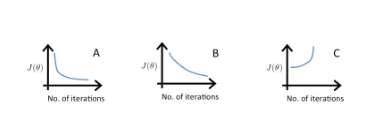
\includegraphics[width=0.9\columnwidth]{ml_figures/convergence.png}

A - good convergence

B - slow convergence

C - learning rate too high

Run GD with $\alpha$ with a range of values with 10-scale factor  3x from previous values

Until you find one value which is too small and one value which is too large

\subsubsection{Momentum}

\subsubsection{Netwon}

\begin{itemize}
\item no learning rate
\end{itemize}

For a function $l$ with the derivative $l^\prime(\theta)$ and second derivative, starting from an initial guess the update rule is:

$\theta := \theta - \frac{l^\prime(\theta)}{l^{\prime\prime}\theta}$

until $l^\prime(\theta)=0$. 

Newton method looks at the approximated tangent to $l(\theta)$ at the point $\theta$ and solves for where the line is equal to 0.

\subsubsection{Newton Raphson Method}

Generalization of Netwon's method to multi-variable / multi dimension settings:

$\theta = \theta - H^{-1}\nabla_\theta l(\theta)$

where $\nabla_\theta$ is a vector of partial derivatives of $l(\theta)$ with respect to $\theta$ and 

$H(\theta)=\frac{\partial^2 l(\theta)}{\partial \theta_i\partial\theta_j}$

Better and faster convergence than GD, but expensive, requires (careful) evaluation, Hessian needs to be invertible (full rank)

Fischer scoring - applying Newton's to logistic regression log likelihood function

\subsection{Polynomial Regression}

Basically, the idea here is to cheat and pre-compute the feature vector. 

For example, $(x_1 := x, x_2 := x^2, x_3 := x^3)$. 

The previous formulation and update rules hold: $\theta^Tx$

In this case it's important to scale the variables!

Other options: sqrt, cubic, squared (which might not fit a lot of models)

\subsection{Normal Equation}

For a feature vector $n$ features and $m$ data points: 

Construct a matrix $X  \in \mathbb{R}^{m\times (n+1)}$ which contains all of features for all the variables + (n+1) column which contains all 1s.

$\left( \begin{matrix} 1 & x_1^1 & ... & x_1^n \\ \vdots & x_2^1 & ... & x_2^n \\   1 & x_m^1 & ... & x_m^n \\ \end{matrix} \right)$

And collect all of the observations in a vector $y \in \mathbb{R}^m $:

And we solve for a model:

$\theta = (X^T X)^{-1} X^T y$



Now, this is true only if $X^T X$ is invertible

Feature scaling is not necc. when using the normal equation.

\subsection{GD vs. Normal Equation}

GD
\begin{itemize}
\item need to choose learning rate
\item need many iterations
\item works well when $n$ is large
\end{itemize}

Normal Equation 
\begin{itemize}
\item slow for large $n$  $O(n^3)$, n=10k is where switching over could be beneficial
\item no need to choose learning rate
\item direct
\end{itemize}

\subsection{When is $X^TX$ non-invertible?}

\begin{itemize}
\item linearly dependent features - i.e. size in $m^2$ and size in feet squared
\begin{itemize}
\item remove features
\end{itemize}
\item too many features $n\ge m$ 
\begin{itemize}
  \item delete features 
  \item use regularization
\end{itemize}
\end{itemize}

\section{Classification}

\subsection{Two Class Problems}
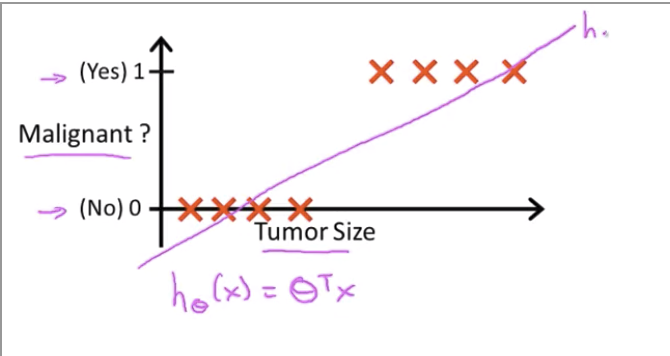
\includegraphics[width=0.9\columnwidth]{ml_figures/log_threshold.png}

Using linear regression model + threshold:

Classification is not actually a linear function - using linear models doesn't work well.

Labels are usually {0,1} known as negative and positive classes.

\subsubsection{Logistic Regression}

Want a model that predict a value $0\le h_\theta(x)\le 1$

Model: $h_\theta(x)=g(\theta^T x)$ 

Logistic/sigmoid function: $g(z) = \frac{1}{1+e^{-z}}$

Together: $h_\theta(x)=\frac{1}{1+e^{-\theta^T x}}$

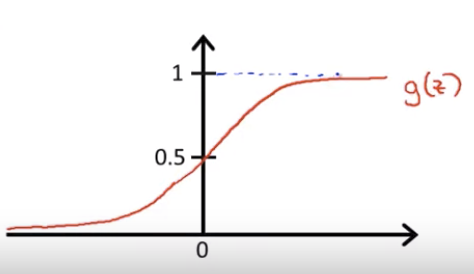
\includegraphics[width=0.9\columnwidth]{ml_figures/sigmoid.png}

Has  asymptotes at {0,1}

\subsubsection{Interpretation of Output}

$h_\theta(x)$ is the estimated probability that  $y=1$ on input $x$ 

$h_\theta(x) = P(y=1|x;\theta)$ 

$P(y=0|x;\theta) = 1-P(y=1|x;\theta)$

\subsubsection{Decision Boundary}

$g(z) \ge 0$.5 when $z>0$ 

$g(\theta^T x ) \ge 0.5$ when $\theta^Tx \ge 0$

(basically, here we  can derive this from $1+e^{-\theta^T x}  = 2$

The decision boundary is a function of the hypothesis and its parameters

\subsubsection{Non Linear Decision Boundaries}

Can perform a similar trick as with linear regression -> polynomial regression - build features such as $x_1^2$ etc...

So for example: 

$$\theta = \left[ \begin{matrix} -1 & 0 & 0  & 1 & 1 \end{matrix} \right]$$

$$h_\theta(x) = g(\theta^T(1,x_1,x_2,x_1^2,x_2^2 )) $$

The decision boundary will lie at $x_1^2 + x_2^2 = 1$

\subsubsection{Cost Function}

Using the linear regression cost function is non convex for the logistic regression.

$Cost(h_\theta(x),y) = \begin{cases} -\log(h_\theta(x))  ;\ \text{if} \;  y=1 \\ -\log(1-h_\theta(x))   ;\ \text{if} \;  y=0  \end{cases}$

This formulation has desirable properties: 

$(h(x)=0, y = 0)$ or$(h(x) = 1, y = 1)$  - cost = 0

Very high penalization if $(h(x)=1, y = 0)$ or$(h(x) = 0, y = 1)$ due to the cost function going asymptotically to $\infty$ :

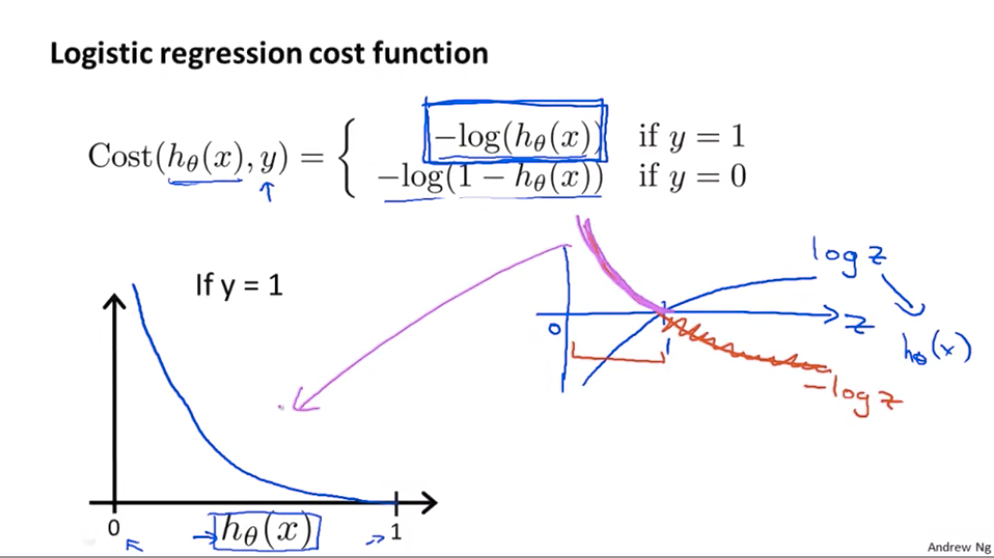
\includegraphics[width=0.8\columnwidth]{ml_figures/cost_function.png}

\subsubsection{Simplified Cost Function}

A generalized cost function is: 

$Cost(h_\theta (x), y) =-y\log(h_\theta(x))-(1-y)\log(1-h_\theta(x))  $

And summarizing over all examples:

$J(\theta)= -\frac{1}{m} \sum_{i=1}^{m} y^{(i)}\log(h_\theta(x^{(i)}))+(1-y^{(i)})\log(1-h_\theta(x^{(i)}))$

To minimize, solve for parameters:

$\min_{\theta} J(\theta) $ 

Output / new prediction: $h_\theta(x) = \frac{1}{1+e^{-\theta^T x}}$

$\frac{\partial}{\partial_{\theta_j}} J(\theta) = \frac 1 m \sum_i (h_\theta(x^{(i)})-y^{(i)})x_j^{(i)}$

Exactly the same update as linear regression. Here the main difference is that $h_\theta$  went from $\theta^T x $ to $\frac{1}{1+e^{-\theta^Tx}}$

And the update rules are:

$\theta_j := \theta_j - \frac{\alpha}{m} \sum_{i=1}^m (h_\theta(x^{(i)}) - y^{(i)}) x_j^{(i)}$

And vectorized:

$\theta:=\theta - \frac{\alpha}{m}X^T(g(X\theta)-\vec{y})$

\subsection{ Maximum Likelihood Estimation + Convexity}

Convexity: gives us lower bounds on the first order approximation of the function (i.e. the first order approximation is guaranteed to be larger than or equal to the real function value).

Assuming that the target variables and input are related via the equation: 

$y^{(i)}=\theta^Tx^{(i)}+\epsilon^{(i)}$

where $\epsilon$ are IID (independently and identically distributed) error terms the captures unmodeled effects, i.e random noise.

Assuming $e^{i}\sim\mathcal{N}(0,\sigma^2)=\frac{1}{\sqrt{2\pi}\sigma}\exp\left(-\frac{(\epsilon^{(i)})^2}{2\sigma^2}\right)$

That implies that: $p(y^{(i)}|x^{(i)};\theta)=\frac{1}{\sqrt{2\pi}\sigma}\exp\left(-\frac{(y^{i}- \theta^Tx^{(i)})^2}{2\sigma^2}\right)$ - this does not depend on $\theta$, the model is not a random variable! 

For the entire model's training set $X$  we can define this the **likelihood** function of the model : $L(\theta)=L(\theta;X;\vec{y})=p(\vec{y}|X;\theta)$

$L(\theta) = L(\theta;X,\vec y) = p(\vec y| X;\theta)$

Since all of the observations are independent:

$L(\theta)= \Pi_{i} p(y^{(i)}| x^{(i)};\theta) = \Pi_{i} \frac{1}{\sqrt{2\pi}\sigma}\exp\left(-\frac{(y^{i}- \theta^Tx^{(i)})^2}{2\sigma^2}\right) $

Maximum likelihood: we should choose a model $\theta$ so as maximize the probability of the data: $\theta$ should maximize $L(\theta)$. 

By deriving the function that maximizes $\log L(\theta)$ , product becomes a series sum and we simply need to maximize the $\frac 1 2 \sum_i (y^{(i)}-\theta^T x^{(i)})^2$ which is the original least-squares cost function.

Note that this does not depend on $\sigma$ !

\subsubsection{Maximum A Posteriori}

/TODO

\subsection{Locally Weighted Linear Models}

\subsection{Optimization Techniques}

There following algorithms are alternatives to GD that do not require choosing a learning rate:

\begin{itemize}
\item Conjugate Gradient
\item BFGS
\item L-BFGS
\end{itemize}

Advantages:
\begin{itemize}
\item No learning rate
\item Faster than GD
\item Line search
\end{itemize}

Disadvantages
\begin{itemize}
\item More complex
\item Prob. don't imp. yourself
\end{itemize}

\subsubsection{Multi-Class Classification Problems}

\subsubsection{One vs. All}

For example: tagging emails according to multiple classes; weather (rainy, sunny)

For each class, train a logistic regression classifier $h_{\theta}^{(i)}(x)$ that predicts that probability that $y=i$.

For new input choose $\max_ih_\theta^i(x)$

\section{ Overfitting vs. Bias}

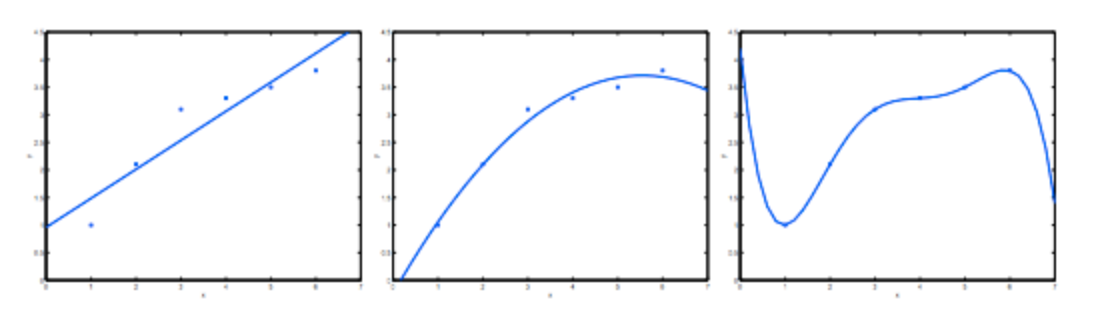
\includegraphics[width=0.5\columnwidth]{ml_figures/overfitting.png}
Underfitting -> high bias.

Overfitting, high variance

High variance - fitting a high order polynomial can be used to fit almost any function, not enough data to give a good hypothesis

If we have too many features, the learned hypothesis may fit the training data very well, but fail to generalize

\subsubsection{Addressing Overfitting}

Reduce number of features

Requires deciding which feature to keep and discard
Model selection algorithms

Regularization

\item keep features but reduce magnitude / values of $\theta_j$ 
\item works well when there are a lot features, each of which contributes less

Modify the cost function by penalizing the parameters:

Penalize higher order parameters: equiv to reducing the model to lower order model - simplfying the model

Penalize all parameters  - trying to keep the hypothesis small, usually corresponds to smoother functions

So now the objective has a data term and a regularization term.

The regularization term: $\lambda\sum_{j=1} \theta_j^2 $ keeps all of them small

If $\lambda $ is very large, in linear reg., all model params will be close to 0 and $h_\theta(x) = \theta_0$  


\section{Measuring Model Performance}

Type 1 Error - False positive - Predict an event when there was no event
Type 2 Error - False negative - Predict no event when in fact there was an event.

\subsubsection{Precision-Recall}

Precision-Recall curves summarize the trade-off between the true positive rate and the positive predictive value for a predictive model using different probability thresholds.

Precision-recall curves are appropriate for imbalanced datasets.

\subsubsection{ ROC -  Receiver Operating Characteristic curve

Summarize the trade-off between the true positive rate and false positive rate for a predictive model using different probability thresholds.

ROC curves are appropriate when the observations are balanced between each class

**Convolution** is a [mathematical operation](https://en.wikipedia.org/wiki/Operation_(mathematics)) on two [functions](https://en.wikipedia.org/wiki/Function_(mathematics)) (*f* and *g*) that produces a third function expressing how the shape of one is modified by the other

$(f\star g)(t) = \int_{-\infty}^{\infty} f(\tau)\cdot g(t-\tau)d\tau = \int_{-\infty}^{\infty} f(t-\tau)\cdot g(\tau)d\tau $

Commutative. 

For functions which only have limited support the integration is only done on the valid domain.

\subsection{L1 vs L2 Norm}

L2 norm strongly penalizes outliers. For good data with some very far outlier it might not generate the "best" fit as judged by a human observer.

L1 favors sparse coefficients.



\section{Support Vector Machines}

https://medium.com/machine-learning-101/chapter-2-svm-support-vector-machine-theory-f0812effc72\section{targetText=A Support Vector Machine (SVM,hyperplane which categorizes new examples.))



\section{Decision Trees}
Recursive repartition of the data

\subsection{Random Forest Regression}

An ensemble of decision trees. During learning tree nodes are split using random variable subset of data features.

All trees vote to produce final result.

For best results trees should be as independent as possible. Splitting using a random subset of features achieves this.

Averaging the product of the trees reduces overfitting to noise

5-100 Trees.

\subsection{Random Fern Regressors}



\section{Boosting}
Learning strong classifiers from weak classifiers.





\section{Naive Bayes Classifier}

/TODO

\section{RANSAC}

A method for dealing with noisy data. 

Partition the method 

Is not determinant, depends on the subset selection, and is not guaranteed to converge.

1. Select a random subset of the original data. Call this subset the *hypothetical inliers*.
2. A model is fitted to the set of hypothetical inliers.
3. All other data are then tested against the fitted model. Those points that fit the estimated model well, according to some model-specific [loss function](https://en.wikipedia.org/wiki/Loss_function), are considered as part of the *consensus set*.
4. The estimated model is reasonably good if sufficiently many points have been classified as part of the consensus set.
5. Afterwards, the model may be improved by reestimating it using all members of the consensus set.

```
Given:
    data – a set of observations
    model – a model to explain observed data points
    n – minimum number of data points required to estimate model parameters
    k – maximum number of iterations allowed in the algorithm
    t – threshold value to determine data points that are fit well by model 
    d – number of close data points required to assert that a model fits well to data

Return:
    bestFit – model parameters which best fit the data (or nul if no good model is found)

iterations = 0
bestFit = nul
bestErr = something really large
while iterations < k {
    maybeInliers = n randomly selected values from data
    maybeModel = model parameters fitted to maybeInliers
    alsoInliers = empty set
    for every point in data not in maybeInliers {
        if point fits maybeModel with an error smaller than t
             add point to alsoInliers
    }
    if the number of elements in alsoInliers is > d {
        % this implies that we may have found a good model
        % now test how good it is
        betterModel = model parameters fitted to all points in maybeInliers and alsoInliers
        thisErr = a measure of how well betterModel fits these points
        if thisErr < bestErr {
            bestFit = betterModel
            bestErr = thisErr
        }
    }
    increment iterations
}
return bestFit
```



\section{Bagging/Boosting}

Collaborative filtering

\section{Generative Models}

\section{Dimension Reduction}

\subsection{PCA}

\chapter{Unsupervised Learning}

Algorithms for finding structure in data.

\section{Clustering}

The clustering problem: given an unlabeled data set, group the data into coherent  subsets or into coherent clusters for us.

\subsection{K Means}

\item $K$ number of clusters + initialization
\item Training set ${x^{(1)},x^{(2)}\dots,x^{(m)}}$
\item $x\in\mathbb{R}^n$
\item By convention, drop $x_0=1$

```
Randomly initialize K cluster centers
While not converged:
1. iterate over data and assign a cluster for each data point based on distance to center
2. re-compute the cluster mean
```

If a cluster becomes empty - remove the cluster

Or randomly re-initialize the cluster

\subsubsection{K Means for Non Separated Clusters}

\subsubsection{K Means Cost Function}

Assuming: 

$c^{(i)}$ index of cluster to which the example $x^{(i)}$ belongs to.

$\mu_k \in \mathbb R ^n $ cluster centroid 

$\mu_{c^{(i)}} \in \mathbb R ^n $ location of the cluster centroid to which example $x^{(i)}$ has been assigned

Example cost for point $Cost(x^{(i)}) = \|x^{(i)} - \mu_{c^{(i)}} \|^2$ 

$J(c^{(1)},\dots, c^{(k)})= \frac{1}{m}\sum_i \|x^{(i)} - \mu_{c^{(i)}} \|^2 $

The objective is to minimize the cost function *distortion* with respect to the clusters (both labelling and centers).

So what k-means algorithm is actually doing is:

1. minimize the cost function with respect to cluster assignments $c^{(i)}$
2. minimize the cost function with respect to cluster centroids $\mu_k$ 

(so basically block coordinate descent?)

\subsubsection{Random Initialization}

\begin{itemize}
\item $K < m$
\item Randomly pick $K$ training examples and set the cluster means to these examples
\end{itemize}

K-mean can get stuck in a local optima - to avoid this a good option is to run k-mean multiple times and get as good global optimum

For multiple initializations - run K-means loads of times, pick the clustering which results in the lowest cost function

This works well for small $K < 10$ .

For large $K$s it is not as effective.

\subsubsection{Number of Clusters - Elbow Method}

Choosing the right K 

Plot the cost function with respect to the number of clusters.![elbow](/Users/kozlovy/Documents/2019_JobApplications/Notes/ml_figures/elbow.png)

In practice it is usually a bit harder, and it is not clear that there is such a transition where the distortion stops.

\section{Dimensionality Reduction}

\subsection{PCA}

PCA is trying to find a lower dimension representation of that data which minimizes the squared distance error of the data from the representation.

Before PCA it is standard practice to perform mean normalization and feature scaling. 

\subsubsection{PCA vs Linear Regression}

<img src="/Users/kozlovy/Documents/2019_JobApplications/Notes/ml_figures/PCA_Linear.png" alt="PCA_Linear" style="zoom:50%;" />

We do not treat $y$ as a special variable

Minimized projected error vs. minimize distance from line

\section{GMM and EM}


\section{Data Generation Using Simulation}

Generating good synthetic data: 
realism, 
diverse,


Want to render images which are as different as possible from each other

Parametric model of humans - procedural generation

\section{Neural Networks}

http://karpathy.github.io/neuralnets/


\section{ML Algorithm Design}

General process of building a ML product:

\begin{enumerate}
\item What is the objective? prediction, recommendation, clustering, search, etc.
\item Pick the right algorithm: supervised vs unsupervised, classification vs regression, generalized linear model / decision tree / neural network / etc.
\item Pick / engineer relevant features based on available data.
\item Pick metrics for model performance.
\item Optionally, comment on how to optimize the model for production.
\end{enumerate}

% %!TEX root = cv_ml_notes.tex
\section{Image Processing}

\subsection{Norms}

$L_1$ norm

$L_2$ norm

Huber’s norm

$L_\infty $

\section{Computational Photography}

Bayer Pattern


\section{Image Analysis}

\textbf{Hough transform} - line representation - line equation and radial.

\subsection{Integral Images}

The value at any point $(x, y)$ in the summed-area table is the sum of all the pixels above and to the left of (*x*, *y*), inclusive where $i(x,y)$  is the value of the pixel at $(x,y)$. The summed-area table can be computed efficiently in a single pass over the image:

$I(x,y) = i(x-1,y-1) + I(x,y-1) + I(x-1,y)-I(x-1,y-1)$

and similarly for any rectangular region:

$ i(A,B,c,D) = I(D) - I(B) - I(C)+I(A)$

\section{ Filtering}

Peak Signal To Noise Ratio 

\begin{itemize}
\item Color Conversion
\item Thresholding
\item Smoothing
\item Morphology
\item Gradient
\end{itemize}

\subsection{Sobel Operator}

Uses $3\times3$ operators which are convolved with the image to compute approximate (center difference?) derivatives in $x$ and $y$ directions.

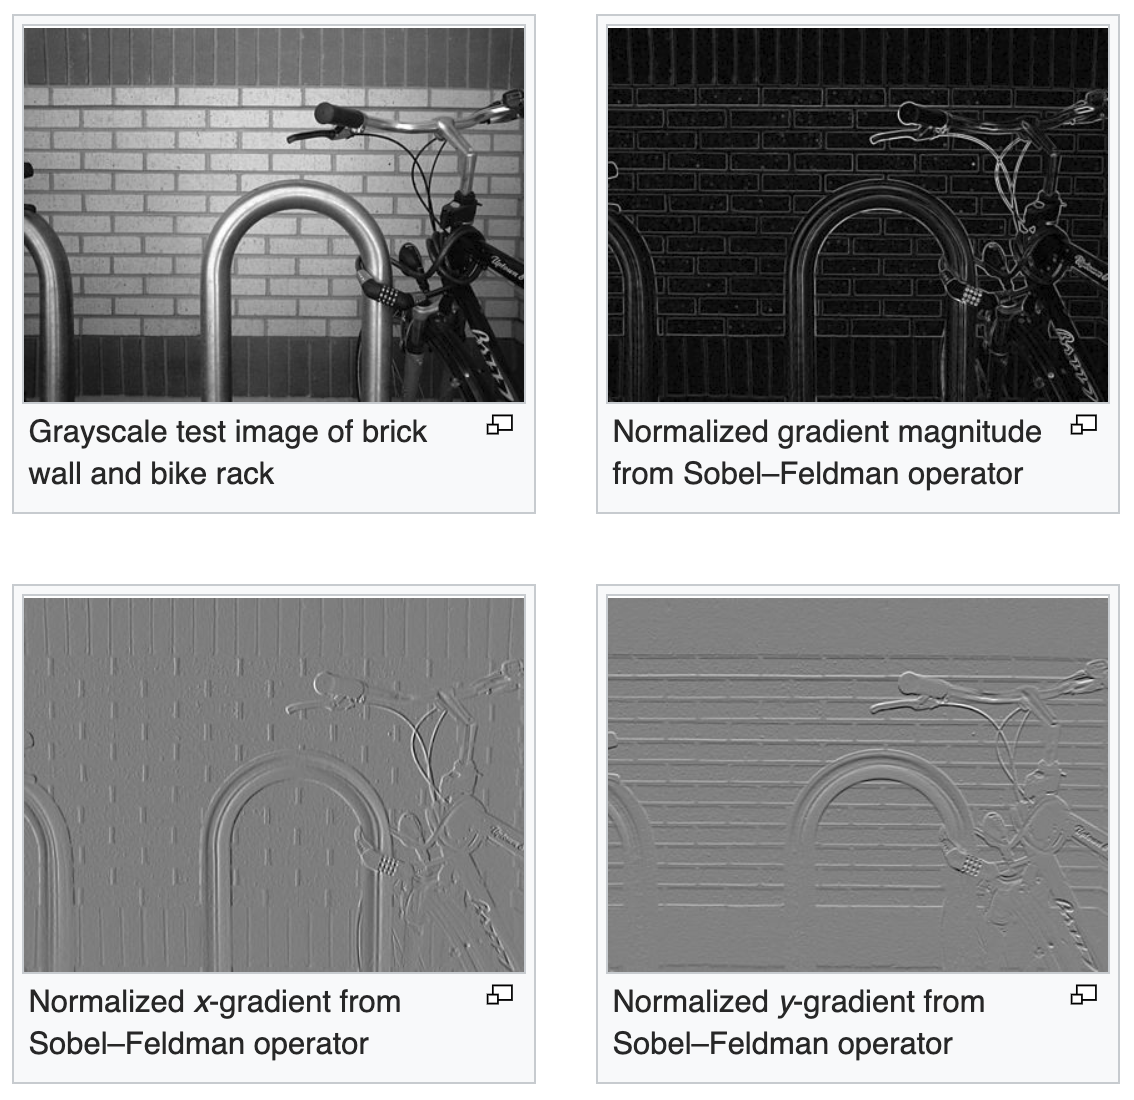
\includegraphics[width=0.9\columnwidth]{img_proc/sobel.png}

\subsection{Canny Edge Detection}
\begin{enumerate}
\item Apply Gaussian filter to smooth the image in order to remove the noise
\item Find the intensity gradients of the image
	The edge orientation is the atan of the intensity of the gradient in each dimension
	The edge magnitude is the sqrt
\item Apply non-maximum suppression to get rid of spurious response to edge detection
\item Apply double threshold to determine potential edges
\item Track edge by hysteresis: Finalize the detection of edges by suppressing all the other edges that are weak and not connected to strong edges.
\end{enumerate}

\textbf{Contours}
\textbf{Histograms}

\subsection{Convolution}

\section{Image Deblurring}

\section{Fourier Transform}

\section{Image Compression}

\section{Optic Flow}

\subsection{Gaussian Pyramids}

Gradient consistency assumption + intensity consistency assumption

Iterative multi scale + warping

Uses an analytic formulation derived from Euler-Lagrange Equations

Results in a dense optic flow field.

Works well for small changes.

\section{Interpolation}

\subsection{Nearest Neighbor}

\subsection{Bilinear Interpolation}

Linear interpolation on a 2D grid. 

\section{Noise Models}

\subsubsection{Salt and Pepper / Black White}
This type of noise happens due to sudden interruption in the image signal.
Also known as data drop noise because statistically its drop the original data values
Can be removed using median or morphological filtering.

\subsubsection{Gaussian noise}
Noise which has a probability density function (PDF) equal to that of the normal distribution.
Can be estimated by taking a dark image and measuring the variance of the pixels. Removed by smoothing.

\section{Semantic Computer Vision} 

Visual Odometry

\section{Silhouette Segmentation / Visual Hull}

\section{Optic Flow}

\section{Image Segmentation / Pixel Labeling}

\section{Object Detection}

\section{Classification Problems}

\section{Event Cameras}

\subsubsection{Features}

\begin{itemize}
\item Low-latency ($\sim1 \mu s$)
\item No motion blur
\item High dynamic range (140 dB instead of 60 dB)
\item Ultra-low power (mean: 1mW vs 1W)
\end{itemize}

Traditional vision algorithms cannot be used because:
\begin{itemize}
\item Asynchronous pixels
\item No intensity information (only binary intensity changes)
\end{itemize}

But they bring new possibilities:
\begin{itemize}
\item Night vision
\item Compact representation and data
\end{itemize}

On static scenes, they mostly produce noise

Main visible features - edges. 

\subsubsection{Linearized Event Generation}

An event is triggered $\log I(x,t) \log I(xt-\Delta t)=\pm C$

Where $C$ is the minimal contrast which is required for triggering an event, scene dependent.

Consider a pixel $p(x,y)$ with gradient $\nabla L(x,y)$ undergoing a motion $u\in(u,v)$ induced by a moving point $p \in\mathbb{R}^3 $

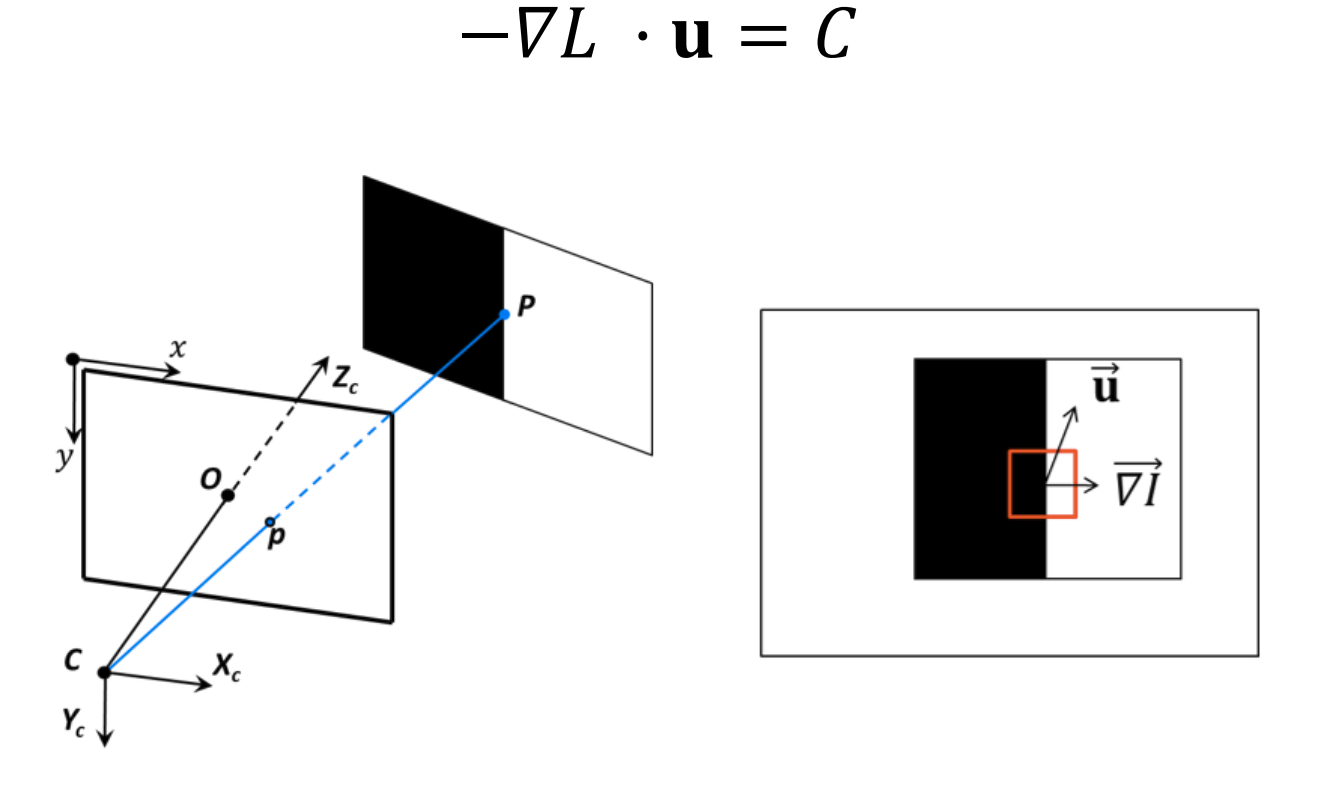
\includegraphics[width=0.9\columnwidth]{event_cameras_fig/event_cameras.png}

From brightness constancy assumption:

$L(x,y,t) = L(x+u,y+v,t+\Delta t)$ from first order approx we get the following $-\nabla L \cdot \vec u = C$

\subsubsection{Deblurring}

A blurry image can be regarded as the integral of a sequence of latent images during the exposure time, while the events indicate the changes between the latent images.

Sharp images are done by subtracting the double integral of the events

\subsubsection{(Sparse) Feature Tracking In Event Space}

\subsubsection{Kanade–Lucas–Tomasi}

Goal: extract features on frames and track them using only events in the blind time between two frames

Uses the event generation model via joint estimation of patch warping and optic flow

Disadvantages: requires GPU for real time tracking and they require knowledge of contract sensitivity, which is scene dependent and differs from pixel to pixel.	

\subsubsection{Image Reconstruction from Event Cameras}

Recurrent neural network (main module: Unet) 

Input: last reconstructed frame + sequences of event tensors (spatio-temporal 3D voxels grid: each voxel contains sum of ON and OFF events falling within the voxel)

Network processes last $N$ events (10,000) 

Trained in simulation only (without seeing a single real image) (we used our event camera simulator: \url{http://rpg.ifi.uzh.ch/esim.html} Noise free simulation with randomized contrast sensitivity.

% \refstepcounter{chapter}
\chapter{Geometry Processing} 

\section{Basics}

Plane normal equation

Plane point distances

Barycentric coordinates


\section{ Surface Representations}

Explicit:
\begin{itemize}
\item Mesh
\item Spline surface
\item Oriented planes
\item Point cloud
\end{itemize}

Implicit - voxel grid:
\begin{itemize}
\item Signed distance fields (implicit) <0, 0, >0
\item Signed distance fields (implicit)
\item Occupancy grid
\item Signed-distance grid
\item Voxel octree
\item Tetrahedral Mesh
\end{itemize}

Volumetric modeling for vision:
• Flexible and robust surface representation
• Handles (changes of) complex surface topologies effortlessly
• Ensures watertight surface / manifold / no self- intersections
• Allows to sample the entire volume of interest by storing information about space opacity
• Voxel processing is often easily parallelizable


Drawbacks:
Implicit surface representation

\subsection{Marching Cubes}
Recovers an isosurface from a volume
ensures a watertight surface
Can be done per voxel
15 combinations of surface intersections per cube
Precise normal specification
Accuracy depends on resolution

Trivial merging or overlapping of different surfaces based on the corresponding implicit functions:
• minimum of the values for merging • averaging for overlapping

Limitations of Marching Cubes
• Maintains 3D entries rather than a 2D surface, i.e.,
higher computational and memory requirements
• Generates consistent topology, but not always the topology you wanted
• Problems with very thin surfaces if resolution not high enough


\section{ICP}

Algorithm:

\section{Point Cloud Merge}

ICP for point cloud matching

Normal Estimation

Outlier detection / removal 

Surface / mesh fitting / template fitting

\subsubsection{Geometric Representations}

Bezier curves

\section{Laplacian Deformation}

% \appendix

% \renewcommand*{\chapterpagestyle}{myappendixpagestyle}

\setcounter{chapter}{0}
\setcounter{figure}{0}

% add your appendix chapters here

%\refstepcounter{chapter}
%\include{appendix}

% \renewcommand*{\chapterpagestyle}{empty}

% \cleardoublepage
% \phantomsection % phantomsection is used here to get the table of contents page numbering right
% \renewcommand\bibname{References}
% \addcontentsline{toc}{chapter}{References}
% \bibliography{bibliography}

% for final version, add CV here

\end{document}

